% ============================================================
% Bachelor Thesis - Technische Hochschule Ingolstadt
% Title: Identification and Interpretation of BMS Signals Through
%        CAN Bus Reverse Engineering on the VW ID. Buzz
% Author: Muhamad Alif Izzuwan Bin Ibrahim
% Layout closely follows the THI reference format.
% ============================================================

\documentclass[11pt,a4paper,oneside,parskip=half]{scrreprt}

% ---------- Encoding / Language ----------
\usepackage[utf8]{inputenc}
\usepackage[T1]{fontenc}
\usepackage[english]{babel}
% ---------- Garamond body font (11 pt, set on the documentclass line) ----------
\usepackage{ebgaramond}              % EB Garamond for the body text
\usepackage[cmintegrals,cmbraces]{newtxmath} % math that pairs with Garamond
\usepackage{microtype}

% ---------- Page geometry (matches reference) ----------
\usepackage[
  a4paper,
  top=2.5cm,
  bottom=2.5cm,
  left=3.0cm,
  right=2.5cm,
  headheight=15pt,
  headsep=0.6cm,
  footskip=1.2cm
]{geometry}

\usepackage{setspace}
\setstretch{1.25}   % 1.25 line spacing

% ---------- Graphics, figures, tables ----------
\usepackage{graphicx}
\graphicspath{{figures/}{fig/}}
\usepackage{float}
\usepackage{caption}
\usepackage{subcaption}
\captionsetup{font=small,labelfont=bf,labelsep=colon,justification=raggedright,singlelinecheck=false}
\captionsetup[table]{justification=centering,singlelinecheck=false}
\captionsetup[figure]{justification=centering,singlelinecheck=false}

\usepackage{booktabs}
\usepackage{tabularx}
\usepackage{longtable}
\usepackage{multirow}
\usepackage{array}
\newcolumntype{C}[1]{>{\centering\arraybackslash}p{#1}}
\newcolumntype{L}[1]{>{\raggedright\arraybackslash}p{#1}}

% ---------- Math & units ----------
\let\Bbbk\relax           % avoid clash between newtxmath and amssymb
\usepackage{amsmath,amssymb}

% ---------- Colour & TikZ ----------
\usepackage[dvipsnames,table]{xcolor}
\usepackage{tikz}
\usetikzlibrary{shapes.geometric,arrows.meta,positioning,calc,fit,matrix,decorations.pathreplacing}

% ---------- Code listings ----------
\usepackage{listings}
\lstset{
  basicstyle=\ttfamily\footnotesize,
  breaklines=true,
  frame=single,
  numbers=left,
  numberstyle=\tiny\color{gray},
  keywordstyle=\bfseries,
  commentstyle=\itshape\color{gray!70!black},
  backgroundcolor=\color{gray!5},
  tabsize=2,
  showstringspaces=false,
  captionpos=b,
  xleftmargin=1em,
  aboveskip=1.2em,
  belowskip=0.6em,
}
\renewcommand{\lstlistingname}{Listing}

% ---------- Headers and footers (reference style) ----------
\usepackage{fancyhdr}

% Define chapter header mark: "CHAPTER 1. INTRODUCTION"
\renewcommand{\chaptermark}[1]{\markboth{CHAPTER \thechapter.\ \MakeUppercase{#1}}{}}
\renewcommand{\sectionmark}[1]{}

\pagestyle{fancy}
\fancyhf{}
\fancyhead[R]{\small\textsc{\leftmark}}
\fancyfoot[L]{\small Muhamad Alif I.~B.~Ibrahim}
\fancyfoot[C]{\small\thepage}
\fancyfoot[R]{\small THI}
\renewcommand{\headrulewidth}{0.5pt}
\renewcommand{\footrulewidth}{0pt}

\fancypagestyle{plain}{%
  \fancyhf{}
  \fancyfoot[L]{\small Muhamad Alif I.~B.~Ibrahim}
  \fancyfoot[C]{\small\thepage}
  \fancyfoot[R]{\small THI}
  \renewcommand{\headrulewidth}{0pt}
}

% ---------- Hyperref (kept plain, black links for print) ----------
\usepackage[hidelinks,
  pdftitle={Identification and Interpretation of BMS Signals Through CAN Bus Reverse Engineering on the VW ID. Buzz},
  pdfauthor={Muhamad Alif Izzuwan Bin Ibrahim},
  pdfsubject={Bachelor Thesis - Technische Hochschule Ingolstadt},
  pdfkeywords={CAN, UDS, OBD-II, BMS, Volkswagen, ID. Buzz, reverse engineering}
]{hyperref}

% ---------- KOMA typography: unbold chapter numbers look plain ----------
\addtokomafont{disposition}{\rmfamily}
\setkomafont{chapter}{\normalfont\bfseries\Large}
\setkomafont{section}{\normalfont\bfseries\large}
\setkomafont{subsection}{\normalfont\bfseries\normalsize}
\RedeclareSectionCommand[beforeskip=-0.5\baselineskip,afterskip=0.35\baselineskip]{chapter}
\RedeclareSectionCommand[beforeskip=1.1\baselineskip,afterskip=0.25\baselineskip]{section}
\RedeclareSectionCommand[beforeskip=0.9\baselineskip,afterskip=0.2\baselineskip]{subsection}

% ---------- Helper macros ----------
\newcommand{\canid}[1]{\texttt{0x#1}}
\newcommand{\udssid}[1]{\texttt{0x#1}}
\providecommand{\hex}{}\renewcommand{\hex}[1]{\texttt{0x#1}}
\newcommand{\byte}[1]{B[#1]}

% ============================================================
\begin{document}
% ============================================================

% ------------------------------------------------------------
% TITLE PAGE (matches reference layout)
% ------------------------------------------------------------
\pagenumbering{roman}
\setcounter{page}{1}
\thispagestyle{empty}

\begin{titlepage}
\thispagestyle{empty}
\begin{center}

% THI logo only, centred

\includegraphics[width=0.45\textwidth]{Technische_Hochschule_Ingolstadt_logo.svg.pdf}

\vspace{1.8cm}

{\large\textbf{Bachelor Thesis}}\\[0.9cm]

% Title
{\LARGE\bfseries Identification and Interpretation of BMS Signals}\\[0.4em]
{\Large\bfseries Through CAN Bus Reverse Engineering}\\[0.2em]
{\Large\bfseries on the Volkswagen ID.~Buzz}\\[1.4cm]

{\normalsize Submitted by}\\[0.6em]
{\Large\bfseries Muhamad Alif Izzuwan Bin Ibrahim}\\[1.4cm]

% Student details block, left-aligned
\begin{flushleft}
\hspace{1.2cm}
\begin{tabular}{@{}p{5.2cm}l@{}}
\textbf{Matriculation number:} & 00124399 \\[2pt]
\textbf{Course of study:}      & Electrical Engineering and Electromobility (B.~Eng.) \\[2pt]
\textbf{Faculty:}              & Electrical Engineering and Computer Science \\
\end{tabular}
\end{flushleft}

\vspace{1.0cm}

\begin{flushleft}
\hspace{1.2cm}
\begin{tabular}{@{}p{5.2cm}l@{}}
\textbf{First examiner:}  & Prof.\ Dr.\ rer.\ nat.\ Hans-Georg Schweiger \\[2pt]
\textbf{Second examiner:} & Prof.\ Dr.\ Werner Huber \\[2pt]
\textbf{Supervisor:}      & Markus Gregor \\
\end{tabular}
\end{flushleft}

\end{center}
\end{titlepage}

% ------------------------------------------------------------
% DECLARATION
% ------------------------------------------------------------
\chapter*{Declaration in accordance with \S18 (4) No.~7 APO THI}
\thispagestyle{plain}
\addcontentsline{toc}{chapter}{Declaration}

\noindent I hereby declare that I have written this thesis independently, that it has not previously been submitted for examination purposes elsewhere, that I have used no sources or aids other than those indicated, and that I have marked verbatim and paraphrased quotations as such.

\vspace{2.5cm}

\noindent
\begin{tabular}{@{}p{7cm}p{7cm}@{}}
\hrulefill & \hrulefill \\[-2pt]
\textbf{Place, Date} \hfill Ingolstadt, 15.07.2026 & \textbf{Signature} \\
\end{tabular}

% ------------------------------------------------------------
% ACKNOWLEDGEMENTS
% ------------------------------------------------------------
\chapter*{Acknowledgements}
\addcontentsline{toc}{chapter}{Acknowledgements}
\thispagestyle{plain}

The present work was carried out as part of my Bachelor studies in Electrical Engineering and Electric Mobility at Technische Hochschule Ingolstadt.

First and foremost, I would like to thank everyone who supported me during the preparation of this thesis. My sincere thanks go to Prof.\ Dr.\ Hans-Georg Schweiger for his weekly supervision and the regular consultation hours that provided invaluable guidance. I also thank Prof.\ Dr.\ Werner Huber for agreeing to act as second examiner and for the constructive feedback he provided on the scope of the work.

I am especially grateful to my supervisor Markus Gregor, who accompanied this work intensively and whose deep knowledge of the research environment shaped the experimental setup around the Volkswagen ID.~Buzz.

Finally, I would like to thank my parents, who believed in me throughout my studies and supported me both financially and morally during the long weeks of data collection and writing.

% ------------------------------------------------------------
% ABSTRACT
% ------------------------------------------------------------
\chapter*{Abstract}
\addcontentsline{toc}{chapter}{Abstract}
\thispagestyle{plain}

The high-voltage traction battery is the most expensive and most safety-critical subsystem of a
battery-electric vehicle, yet the mapping from its internal state to the bytes on the vehicle bus is
proprietary. On the Volkswagen MEB platform the raw battery-management broadcast frames are not
reachable at the diagnostic connector: a central gateway separates the private powertrain networks
from the OBD-II bus. This thesis therefore acquires the battery state \emph{actively}, by issuing
Unified Diagnostic Services \texttt{ReadDataByIdentifier} requests from a CANedge2 data logger
connected to the OBD-II port of a Volkswagen ID.~Buzz, so that requests and responses are captured in
one hardware-timestamped recording without a second tester on the bus.

The identifiers and their proposed encodings are not derived from scratch. They are taken from a
publicly circulating diagnostic identifier list compiled for the closely related VW~ID.3
(\cite{vwmebpidlist}), which is treated here as an unverified hypothesis rather than a specification.
The contribution of this work is therefore threefold: to establish which of those identifiers the
ID.~Buzz answers at all through its gateway, to test each proposed encoding against the physical
state of the vehicle and against the internal consistency of the decoded set, and to recover those
encodings the list omits or states incorrectly.

Of 60~identifiers requested per cycle across four control units, 52 returned a positive single-frame
response, of which 49 carried a usable value; six were truncated to their first frame because the
logger's transmit engine implements no ISO-TP segmentation, and two were never answered. The decoded
pack voltage (373.25--373.75~V), the 28~sampled cell voltages (3.888--3.890~V, inter-cell spread
2.8~mV) and the pack temperatures (16.0--16.4~\textdegree C) are mutually consistent and reproducible
across three independent sessions. Three findings go beyond the source list: the raw code
\texttt{0x0FFE} is identified as a reserved \emph{not-available} marker returned by unpopulated cell
slots; the leading bytes of the cell-extreme identifiers are shown to carry the cell voltage scaled by
$1/4096$; and the pack is shown, by three independent lines of evidence, to expose exactly
96~cell-voltage channels. The limits of the method are stated explicitly: all recordings were taken
with the vehicle drive-ready but stationary, so current- and power-related identifiers never left
their idle value, and only two signals could be validated against a reference genuinely independent of
the bus.

% ------------------------------------------------------------
% CONTENTS / LOF / LOT
% ------------------------------------------------------------
\tableofcontents
\addcontentsline{toc}{chapter}{Contents}

\listoffigures
\addcontentsline{toc}{chapter}{List of Figures}

% ------------------------------------------------------------
% ABBREVIATIONS
% ------------------------------------------------------------
\chapter*{Abbreviations}
\addcontentsline{toc}{chapter}{Abbreviations}

\begin{tabular}{@{}lp{10.5cm}@{}}
\textbf{BEV}   & Battery Electric Vehicle \\
\textbf{BMC}   & Battery Management Controller \\
\textbf{BMS}   & Battery Management System \\
\textbf{CAN}   & Controller Area Network (ISO 11898) \\
\textbf{CAN-FD}& CAN with Flexible Data-rate \\
\textbf{CF}    & Consecutive Frame (ISO-TP) \\
\textbf{CSC}   & Cell Supervision Circuit \\
\textbf{DID}   & Data Identifier (UDS) \\
\textbf{DoCAN} & Diagnostic communication over CAN \\
\textbf{ECU}   & Electronic Control Unit \\
\textbf{EOBD}  & European On-Board Diagnostics \\
\textbf{FC}    & Flow Control frame (ISO-TP) \\
\textbf{FF}    & First Frame (ISO-TP) \\
\textbf{HV}    & High Voltage \\
\textbf{ISO-TP}& ISO 15765-2 Transport Protocol \\
\textbf{LSB}   & Least Significant Bit (here: quantisation step) \\
\textbf{MDF}   & Measurement Data Format (ASAM MDF 4.11, file extension MF4) \\
\textbf{MEB}   & Modularer E-Antriebs-Baukasten (Modular Electric Drive Matrix) \\
\textbf{NRC}   & Negative Response Code (UDS) \\
\textbf{OBD-II}& On-Board Diagnostics, second generation (SAE J1962) \\
\textbf{PCI}   & Protocol Control Information (ISO-TP) \\
\textbf{PTC}   & Positive Temperature Coefficient (heater) \\
\textbf{SF}    & Single Frame (ISO-TP) \\
\textbf{SID}   & Service Identifier (UDS) \\
\textbf{SNA}   & Signal Not Available (reserved sentinel code) \\
\textbf{SOC}   & State of Charge \\
\textbf{SOH}   & State of Health \\
\textbf{UDS}   & Unified Diagnostic Services (ISO 14229) \\
\end{tabular}

\clearpage
\pagenumbering{arabic}
\setcounter{page}{1}

% ============================================================

\chapter{Introduction}
% ============================================================
The high-voltage battery of an electric vehicle continuously computes a detailed picture of its own state, and almost none of that picture is meant to leave the car. This chapter explains why that data is worth reaching, why the obvious route to it is closed on the Volkswagen MEB platform, and which route remains open. It closes with the four research questions against which the rest of the work is assessed.

\section{Motivation}
Electric mobility has moved from a niche segment to a central pillar of the automotive industry, and in every battery-electric vehicle the high-voltage traction battery is the most expensive and most safety-critical subsystem. Its internal state -- state of charge (SOC), pack voltage and current, individual cell voltages and cell temperatures -- governs the range available to the driver, the long-term reliability of the vehicle and its residual value, and is continuously estimated and supervised by a dedicated battery management system (BMS). For anyone assessing a used electric vehicle, monitoring a fleet, or investigating battery safety in a research context, access to those internal parameters is of central importance.

This information travels inside the vehicle over the Controller Area Network (CAN)~\cite{iso11898}. Its frames are freely observable on the physical layer, but the semantic layer is not: the manufacturer databases that map raw bytes onto volts, amperes and degrees Celsius are proprietary and are not released. Without them a recording is a stream of hexadecimal bytes -- one sees \emph{that} a message arrives, but not \emph{what} it means. Closing that gap is the task of reverse engineering.

Two routes lead to it. \textit{Passive} reverse engineering taps the bus on which the BMS broadcasts and infers each byte's meaning statistically from recorded traffic; it presupposes access to that bus. On the Volkswagen Modular Electric Drive Matrix (MEB) platform that precondition is not met at the diagnostic connector, because a central gateway electronic control unit (ECU) separates the private powertrain and battery networks from it, and reaching them physically would mean invasively tapping high-voltage wiring -- impractical and unsafe on a production vehicle. \textit{Active} diagnostic reverse engineering asks rather than listens. Through the standardised Unified Diagnostic Services (UDS)~\cite{iso14229}, carried over ISO~15765-2~\cite{iso15765} and reached through the OBD-II connector~\cite{saej1962}, Data Identifiers (DIDs) can be requested directly from the battery ECU: the gateway does not relay the raw broadcasts, but it does route addressed diagnostic requests inward and return the answers. The very isolation that closes the passive route leaves a legitimate, standardised one open -- the data is reached not by listening, but by requesting.

Reaching it is not the same as understanding it. Volkswagen publishes neither the identifiers nor their encodings, but the closely related VW~ID.3 has been characterised by the independent diagnostics community, and a publicly circulating identifier list~\cite{vwmebpidlist} proposes a byte layout and a linear scaling for many manufacturer-specific DIDs. That list is undocumented, unvalidated and compiled for a different vehicle: it is a hypothesis, not a specification. This thesis applies the active approach to a Volkswagen ID.~Buzz -- a high-volume MEB vehicle whose gateway topology, diagnostic addressing and battery-management concept are representative of a large family of Volkswagen Group BEVs -- in order to establish which of those identifiers the vehicle actually answers, whether the proposed encodings survive the transfer, and which of them must be recovered or corrected from the measurements themselves.

\section{Problem Statement}
\label{sec:problem}
The main goal of this thesis is to reverse engineer the high-voltage battery signals of a Volkswagen ID.~Buzz through its OBD-II diagnostic port. Because the raw BMS broadcast bus is isolated by the central gateway and its frames never reach the diagnostic connector, the work cannot rely on passively observing traffic. It instead focuses on actively requesting battery Data Identifiers through the UDS protocol and recovering their physical meaning from the raw response bytes. The primary deliverable is a demonstrated, repeatable capability to request and correctly decode the key high-voltage battery parameters -- in particular the state of charge, the pack voltage, the individual cell voltages and the cell-temperature statistics -- and to confirm each of them against the physical state of the vehicle rather than accepting it on faith.

Achieving this goal requires bridging several gaps at once. It must first be established what is actually reachable from the OBD-II connector and why, so that the effort is directed at services and identifiers that the gateway will genuinely answer. The set of relevant Data Identifiers must then be selected and requested within the practical constraints of the available logging hardware. Finally, and most demandingly, the undocumented byte layouts and scalings must be reconstructed and their correctness demonstrated against independent physical references. Within this overall objective the work addresses the following research questions:

\begin{enumerate}
  \item Which CAN bus is exposed on the OBD-II connector of the Volkswagen ID.~Buzz, and why are the raw BMS broadcast frames not directly observable on it?
  \item Which UDS services and Data Identifiers of the battery management ECU are reachable through the gateway from the OBD-II connector without a security-access unlock?
  \item How can the byte layout and scaling of these undocumented, manufacturer-specific DIDs be reverse engineered into physical battery parameters?
  \item How well do the decoded UDS values agree with the physical reference values of the test vehicle (dashboard SOC, measured pack voltage, ambient temperature), and where does the method reach its limits?
\end{enumerate}

Taken together, these four questions trace the path from the electrical architecture of the vehicle, through the diagnostic protocol stack, to a set of validated physical battery parameters, and they define the scope against which the results of this thesis are ultimately assessed.

\section{Structure of the Thesis}
This thesis is divided into six main chapters, which follow the natural progression from background, through method, to results, discussion and conclusion.

Chapter~1 gives an overview of the task, the motivation and the structure of the thesis, and it defines the research questions that the remainder of the work sets out to answer.

Chapter~2 presents the theoretical background by means of a literature review. It covers the CAN bus protocol, the OBD-II connector, the ISO-TP transport protocol and the UDS application layer as the communication foundation, and then turns to the Volkswagen MEB platform, traction-battery management systems in BEVs and the state of the art of CAN bus reverse engineering. Together these topics provide the vocabulary and the technical context needed to follow the practical work.

Chapter~3 describes the materials and methods used in this work. The test vehicle, the CANedge2 data logger, the OBD-II connection and the software tool chain based on \texttt{asammdf} and Python are documented, together with the UDS-based reverse-engineering methodology and the detailed reasoning for using active diagnostics rather than passive bus tapping.

Chapter~4 presents the results: the UDS logging campaign, the response coverage across the requested Data Identifiers, and the battery parameters decoded from the BMS and validated against the physical state of the vehicle.

Chapter~5 discusses the findings. The limitations of the approach and the comparison with related work are analysed, and practical applications of the method are outlined.

Chapter~6 concludes the work and gives an outlook on future research directions.

% ============================================================

% ============================================================
\chapter{Fundamentals and State of the Art}
% ============================================================
In this chapter the essential fundamentals for understanding this work are explained. The introduction serves to describe the Controller Area Network, the layered diagnostic protocol stack built on top of it (ISO-TP and UDS), the OBD-II interface, the Volkswagen MEB platform and the battery management subsystem of a modern BEV. Each of these building blocks is introduced not in isolation but with an eye to the specific question this thesis pursues, namely how the internal state of a high-voltage traction battery can be observed from the outside of the vehicle. Understanding why the raw battery signals are difficult to reach, and why an active diagnostic query is nonetheless able to retrieve them, requires a clear picture of how the individual layers of the in-vehicle network cooperate. The chapter therefore proceeds from the electrical bottom of the stack upwards to the application layer, then places the battery subsystem into the context of the MEB vehicle architecture, and finally closes with a short review of prior art in automotive CAN reverse engineering.

\section{Controller Area Network (CAN)}
The Controller Area Network was originally developed by Bosch in the 1980s and is today standardised in ISO 11898~\cite{iso11898}. It was conceived to replace the ever-growing bundle of dedicated point-to-point wires in a vehicle with a single shared serial medium, so that any number of electronic control units (ECUs) could exchange information over one twisted pair rather than over an individual harness for each signal. This change was driven by the sharp rise in the number of ECUs in passenger cars during that decade and by the associated weight, cost and reliability penalty of a purely point-to-point wiring scheme. CAN answered this need with a design that is deliberately simple at the node level yet robust at the system level.

It is a serial, differential, multi-master broadcast bus that has become the backbone of automotive embedded networking. Every message is transmitted to all nodes simultaneously; there is no central bus master and no addressing of a specific recipient. Instead, each message carries an identifier that describes the \emph{content} of the message rather than its destination, and each receiving node decides autonomously, by filtering on that identifier, whether the message is relevant to it. Its key properties -- bit-wise, non-destructive arbitration, short message length, high reliability through CRC protection and low hardware cost -- make it extremely well suited to the distributed control problem of a modern vehicle. The combination of content-based addressing, deterministic priority resolution and strong error detection is precisely what allows dozens of independently developed ECUs to share one medium without a coordinating master, and it is the reason CAN has remained the dominant in-vehicle network for several decades despite the arrival of faster alternatives.

\subsection{Physical and Link Layer}
On the physical layer, CAN uses a twisted differential pair (CAN-H and CAN-L) terminated with 120~$\Omega$ resistors at both ends. Signalling differentially -- that is, encoding each bit as the voltage difference between the two lines rather than as an absolute voltage against ground -- gives the bus a high immunity to electromagnetic interference, because any noise coupled into the harness affects both conductors almost equally and is cancelled when the receiver evaluates the difference. The termination resistors match the characteristic impedance of the cable and suppress the signal reflections that would otherwise corrupt the sharp bit edges on a bus that may be several metres long inside a vehicle.

The bus is driven by each node through a transceiver that produces two complementary states: a \textit{dominant} state (logical 0) and a \textit{recessive} state (logical 1). The naming is literal: when one node drives the bus dominant while another drives it recessive, the dominant level prevails, so the bus behaves electrically like a wired-AND of all connected transmitters. A dominant bit always overrides a recessive one, which is the key mechanism for the arbitration scheme described below. Because every node reads back the actual bus level while it transmits, this same wired-AND behaviour is also used for bit-wise error detection and acknowledgement, not only for arbitration. For in-vehicle networks, bit rates of 500~kbit/s (high-speed CAN for powertrain) and 100~kbit/s (comfort CAN) are the most common values in the Volkswagen Group; the higher rate is reserved for the time-critical powertrain and chassis domains, where control loops demand short and predictable message latencies, while the lower rate is sufficient for comfort and body functions that tolerate more delay.

\subsection{Frame Structure}
Every CAN message is transmitted as a frame with the structure shown in Figure~\ref{fig:can_frame}. Apart from the start-of-frame bit, an 11-bit arbitration identifier (or 29-bit extended identifier), and control bits, the frame carries a payload of up to 8~bytes (Classical CAN; CAN-FD supports up to 64~bytes) protected by a 15-bit CRC followed by a recessive CRC delimiter, so the CRC field occupies 16~bit in total. The individual fields each serve a distinct purpose: the single dominant start-of-frame bit synchronises all receivers to the beginning of a transmission; the identifier field both names the message content and, as explained in the next subsection, decides its priority; the control field encodes the data length code that tells receivers how many payload bytes follow; the data field carries the actual application information; the CRC field allows every receiver to verify the integrity of the frame; and the acknowledgement slot lets any correctly receiving node signal success back to the transmitter.

\begin{figure}[H]
\centering
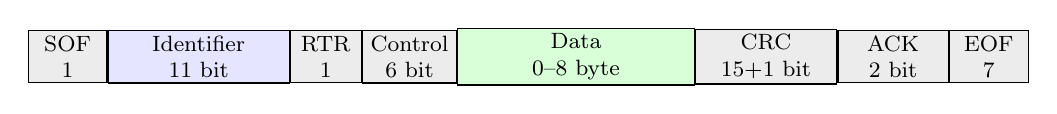
\begin{tikzpicture}[
  every node/.style={draw,minimum height=1.3em,font=\footnotesize,
    inner sep=2pt, align=center}]
\node[fill=gray!15,minimum width=1.0cm] (sof) {SOF\\1};
\node[right=0pt of sof,fill=blue!10,minimum width=2.3cm]  (id)  {Identifier\\11 bit};
\node[right=0pt of id,fill=gray!15,minimum width=0.9cm] (rtr) {RTR\\1};
\node[right=0pt of rtr,fill=gray!15,minimum width=1.2cm] (ctrl){Control\\6 bit};
\node[right=0pt of ctrl,fill=green!15,minimum width=3.0cm](data){Data\\0--8 byte};
\node[right=0pt of data,fill=gray!15,minimum width=1.8cm] (crc) {CRC\\15+1 bit};
\node[right=0pt of crc,fill=gray!15,minimum width=1.4cm] (ack) {ACK\\2 bit};
\node[right=0pt of ack,fill=gray!15,minimum width=1.0cm] (eof) {EOF\\7};
\end{tikzpicture}
\caption{Simplified layout of a classical CAN 2.0A data frame. The identifier field is used for bitwise arbitration; the data field carries the payload the application layer is interested in.}
\label{fig:can_frame}
\end{figure}

To prevent the transmitter and receivers from losing bit synchronisation during long runs of identical bits, CAN applies \textit{bit stuffing}: after five consecutive bits of the same polarity the transmitter inserts one bit of the opposite polarity, which the receivers remove again. This mechanism, together with the CRC and the acknowledgement slot, is part of the extensive error-handling machinery that gives CAN its characteristic robustness. The distinction between the 11-bit standard identifier (CAN~2.0A) and the 29-bit extended identifier (CAN~2.0B) is important for this thesis: ordinary broadcast traffic and many gateway ECUs use the shorter 11-bit form, whereas the addressed diagnostic exchange with the battery ECU relies on 29-bit extended identifiers, as detailed in Section~\ref{ssec:diag_addr}.

\subsection{Arbitration and Prioritisation}
CAN uses Carrier-Sense Multiple Access with Collision Resolution (CSMA/CR). When two or more nodes start transmitting simultaneously, each node reads back the bus level during its own transmission. Because a dominant bit (0) always wins over a recessive bit (1), the node with the numerically lower identifier automatically continues to transmit while the others switch to the listen state. The essential feature is that this collision resolution is \emph{non-destructive}: unlike Ethernet's classical CSMA/CD, where a collision destroys all colliding frames and forces a random back-off, CAN loses no information at all, because the winning message continues on the bus without interruption while the losing nodes seamlessly become receivers of that very message. This guarantees that the highest-priority message is never delayed by a collision.

A concrete walk-through makes the mechanism tangible. Suppose two nodes contend for the bus at the same time, one wishing to send identifier \canid{100} and the other \canid{101}. After the shared start-of-frame bit, both nodes begin to clock out their 11-bit identifiers most-significant-bit first, and because the leading bits of \hex{100} and \hex{101} are identical, both keep transmitting and both keep reading the bus without any disagreement. The two identifiers differ only in their least-significant bit: the first node drives a dominant 0 there, while the second drives a recessive 1. At that bit time the bus therefore settles to the dominant level. The second node, reading back the bus, sees a dominant 0 where it transmitted a recessive 1, recognises that it has lost arbitration, and immediately stops transmitting to become a receiver. The first node, whose transmitted bit matches the bus, notices nothing unusual and simply carries on sending the rest of its frame. No time is lost, no frame is corrupted, and the lower-numbered identifier has silently won. In an electric vehicle, safety-critical messages (such as the motor torque request or the battery current measurement) are therefore assigned low arbitration IDs, while convenience signals use higher IDs.

\subsection{Classical CAN vs.\ CAN-FD}
Two variants of the protocol are relevant. \textit{Classical CAN} (CAN~2.0, ISO~11898-1:2003) is limited to 8~payload bytes per frame and a single bit rate for the whole frame. \textit{CAN-FD} (CAN with Flexible Data-rate, standardised in ISO~11898-1:2015) extends this in two ways: the payload grows to up to 64~bytes, and the data phase of the frame may be transmitted at a higher bit rate than the arbitration phase, while the arbitration mechanism itself is unchanged. The motivation for CAN-FD was the growing bandwidth demand of modern vehicles: larger payloads reduce the protocol overhead per useful byte, and switching to a faster bit rate during the data phase -- once arbitration has already selected a single transmitter and the bit-wise, propagation-limited contention is over -- shortens the time the bus is occupied by each message. Crucially, because the arbitration phase is untouched, CAN-FD preserves the deterministic, priority-based bus access that makes Classical CAN attractive in the first place.

The diagnostic CAN bus exposed on the OBD-II connector of the ID.~Buzz operates as a \textbf{Classical CAN bus at 500~kbit/s with 11-bit broadcast identifiers}; the diagnostic exchange with the battery ECU additionally uses 29-bit extended identifiers (Section~\ref{ssec:diag_addr}). It is \emph{not} CAN-FD. This is the decisive constraint behind the methodology of this thesis: because each frame carries at most 8~bytes, every UDS response longer than 7~payload bytes must be segmented by ISO-TP, and a logger that can only emit single CAN frames cannot read those multi-frame identifiers (Section~\ref{sec:uds_procedure}). The data logger used here (CANedge2)~\cite{csselectronics_canedge2} electrically supports both Classical CAN and CAN-FD, but is configured for Classical CAN at 500~kbit/s to match the vehicle, with the CAN-FD data bit rate left defined (2~Mbit/s) only so that the controller can initialise. This single-frame limitation is not a peripheral detail but the central reason why some multi-byte identifiers can only be partially recovered in this work, and it motivates the deliberately selective, single-frame UDS strategy developed in the following chapters.

\section{Diagnostics: OBD-II, ISO-TP and UDS}
While the CAN bus is the low-level transport medium, automotive diagnostics rely on two additional layers built on top of CAN: a transport protocol that allows messages longer than 8~bytes to be fragmented and reassembled (ISO-TP), and an application layer that defines services, sub-functions and data identifiers (UDS). Both are accessed from outside the vehicle via a standardised connector: the OBD-II port. Together these three elements form a clean division of labour, in which each layer solves exactly one problem and hides its internal complexity from the layer above -- the physical connector standardises access, the transport layer standardises segmentation, and the application layer standardises the meaning of the exchanged data.

It is useful to locate each of these protocols in the OSI reference model before going into detail, because the rest of the thesis repeatedly refers to ``which layer'' a given problem belongs to. The diagnostic stack used here maps onto the OSI layers as summarised in Table~\ref{tab:osi_stack}: CAN occupies the two lowest layers, ISO-TP provides the network/transport function that classical CAN itself lacks, and UDS is the application protocol that the battery management ECU actually speaks. Thinking in terms of layers is not merely pedagogical bookkeeping: the single-frame limitation discussed above is a transport-layer problem, whereas the interpretation of an unknown data identifier is an application-layer problem, and keeping the two separate is what allows the methodology to reason precisely about where a given difficulty originates.

\begin{table}[H]
\caption{Mapping of the diagnostic protocol stack used in this thesis onto the OSI reference model.}
\label{tab:osi_stack}
\centering
\begin{tabular}{clp{6.6cm}}
\toprule
\textbf{OSI layer} & \textbf{Protocol} & \textbf{Role in this work} \\
\midrule
7 -- Application & UDS (ISO 14229)        & Services, sub-functions and Data Identifiers; \hex{22} \textit{ReadDataByIdentifier} returns the battery parameters. \\
6/5             & (not used)              & No presentation/session layer in CAN diagnostics. \\
4/3 -- Transport/Network & ISO-TP (ISO 15765-2) & Segments UDS messages longer than 7~bytes into First/Consecutive frames and reassembles them. \\
2 -- Data link  & CAN (ISO 11898-1)       & Frame format, arbitration, CRC, acknowledgement. \\
1 -- Physical   & CAN (ISO 11898-2)       & Differential CAN-H/CAN-L pair, 500~kbit/s, 120~$\Omega$ termination. \\
\bottomrule
\end{tabular}
\end{table}

\subsection{The OBD-II Connector (SAE J1962)}
All passenger cars sold in the European Union must expose a 16-pin diagnostic connector in the driver's footwell area, standardised by SAE~J1962~\cite{saej1962}. The European on-board diagnostics (EOBD) requirement was introduced by Directive~98/69/EC~\cite{eudir9869} for new petrol passenger cars from 2000 (type approval) and 2001 (first registration), and extended to diesel passenger cars by Directive~2001/1/EC~\cite{eudir20011} from 2003 and 2004 respectively. The connector was originally mandated to make emission-related diagnostics uniformly accessible across manufacturers, so that a standard scan tool could read fault codes and emission parameters from any compliant vehicle without proprietary hardware. Two pins carry the high-speed CAN bus used for emissions diagnostics (pin~6 = CAN-H, pin~14 = CAN-L). On many manufacturers' vehicles, additional pins are used by a \textit{gateway ECU} that multiplexes private manufacturer buses onto the OBD-II connector only for authenticated diagnostic tester sessions. This gateway is central to the present work: it is precisely because the gateway does not forward the raw internal battery broadcast traffic to the OBD-II connector that a passive recording at the port cannot see the battery frames directly, and it is precisely because the gateway \emph{does} route addressed diagnostic requests inward to the battery ECU that an active query can still reach the data.

The physical interface is also what powers the measurement setup used later in this thesis. Beyond the two CAN pins, the connector provides a permanent supply and ground that allow a self-contained logger to draw its operating current directly from the vehicle without any separate power source. The pins relevant to this work are summarised in Table~\ref{tab:obd2_pins}.

\begin{table}[H]
\caption{Key pins of the SAE~J1962 OBD-II connector used in this thesis.}
\label{tab:obd2_pins}
\centering
\begin{tabular}{llp{7cm}}
\toprule
\textbf{Pin} & \textbf{Signal} & \textbf{Function} \\
\midrule
4  & Chassis ground           & Vehicle chassis reference. \\
5  & Signal ground            & Signal return. \\
6  & CAN-H (HS-CAN)           & High-speed CAN 500~kbit/s, used for OBD-II and UDS. \\
14 & CAN-L (HS-CAN)           & Complementary line to pin~6. \\
16 & Battery positive         & Permanent +12~V from the vehicle battery (used by the data logger). \\
\bottomrule
\end{tabular}
\end{table}

\subsection{ISO 15765-2 Transport Protocol}
A single classical CAN frame can carry only up to 8~bytes. UDS responses for an identifier such as ``read VIN'' or ``read DID'' routinely need more than 8~bytes. The ISO 15765-2 transport protocol~\cite{iso15765} solves this by fragmenting the application-layer PDU into multiple CAN frames of four possible types: \textit{Single Frame} (SF) for up to 7 bytes of payload, \textit{First Frame} (FF) plus a sequence of \textit{Consecutive Frames} (CF) for longer messages, and \textit{Flow Control} (FC) frames for sender throttling. The first byte (or first nibble) of each ISO-TP frame is a protocol-control-information (PCI) field that encodes the frame type and, depending on the type, either the total message length or the sequence number of the fragment, so that the receiver can distinguish the four cases and reassemble the fragments in the correct order.

\begin{figure}[H]
\centering
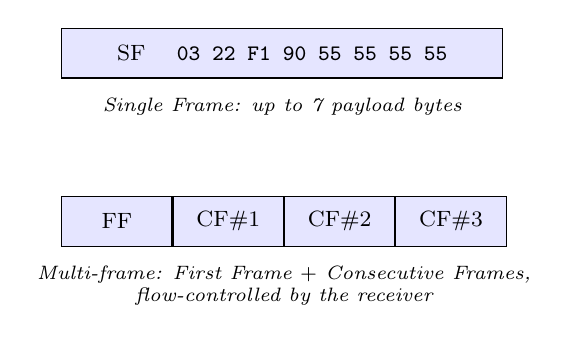
\begin{tikzpicture}[
  font=\footnotesize,
  tx/.style={draw,fill=blue!10,minimum height=1.8em,inner sep=3pt,align=center},
  ftxt/.style={font=\scriptsize\itshape,align=center}]

% --- single frame: one box, 4 x 1.4 cm wide so the two rows align ---
\node[tx,minimum width=5.6cm] (sf) {SF \quad \texttt{03 22 F1 90 55 55 55 55}};
\node[ftxt,below=1.2mm of sf] (sfc) {Single Frame: up to 7 payload bytes};

% --- multi frame: four boxes spanning exactly the same 5.6 cm ---
\node[tx,minimum width=1.4cm,anchor=north west] (ff)  at ([yshift=-9mm]sfc.south -| sf.west) {FF};
\node[tx,minimum width=1.4cm,right=0pt of ff]  (cf1) {CF\#1};
\node[tx,minimum width=1.4cm,right=0pt of cf1] (cf2) {CF\#2};
\node[tx,minimum width=1.4cm,right=0pt of cf2] (cf3) {CF\#3};
\node[ftxt,below=1.2mm of cf1.south east]
  {Multi-frame: First Frame $+$ Consecutive Frames,\\flow-controlled by the receiver};
\end{tikzpicture}
\caption{ISO 15765-2 (ISO-TP) protocol data units. Short diagnostic messages fit in a Single Frame; longer responses use First Frame + Consecutive Frames with Flow Control.}
\label{fig:isotp}
\end{figure}

The temporal interplay of these frame types between the diagnostic client (tester) and the server (ECU) is shown in Figure~\ref{fig:isotp_seq}. The tester opens the exchange with a Single Frame request; the ECU answers with a First Frame, waits for the tester's Flow Control frame and then streams the Consecutive Frames, spaced by the minimum separation time \texttt{STmin} requested in the Flow Control frame. The Flow Control frame is what makes segmentation reliable across devices of different speed: it lets the receiver dictate both the block size, that is how many Consecutive Frames it will accept before it must be polled again, and the \texttt{STmin} gap that the sender must insert between successive frames so that a slower receiver is never overrun. This dialogue is only possible if the requesting device is itself capable of sending a Flow Control frame in response to a First Frame; a logger that can emit nothing but a single, periodically repeated request frame cannot complete the handshake, which is the direct reason why multi-frame identifiers are recovered only as their First Frame in this work.

\begin{figure}[H]
\centering
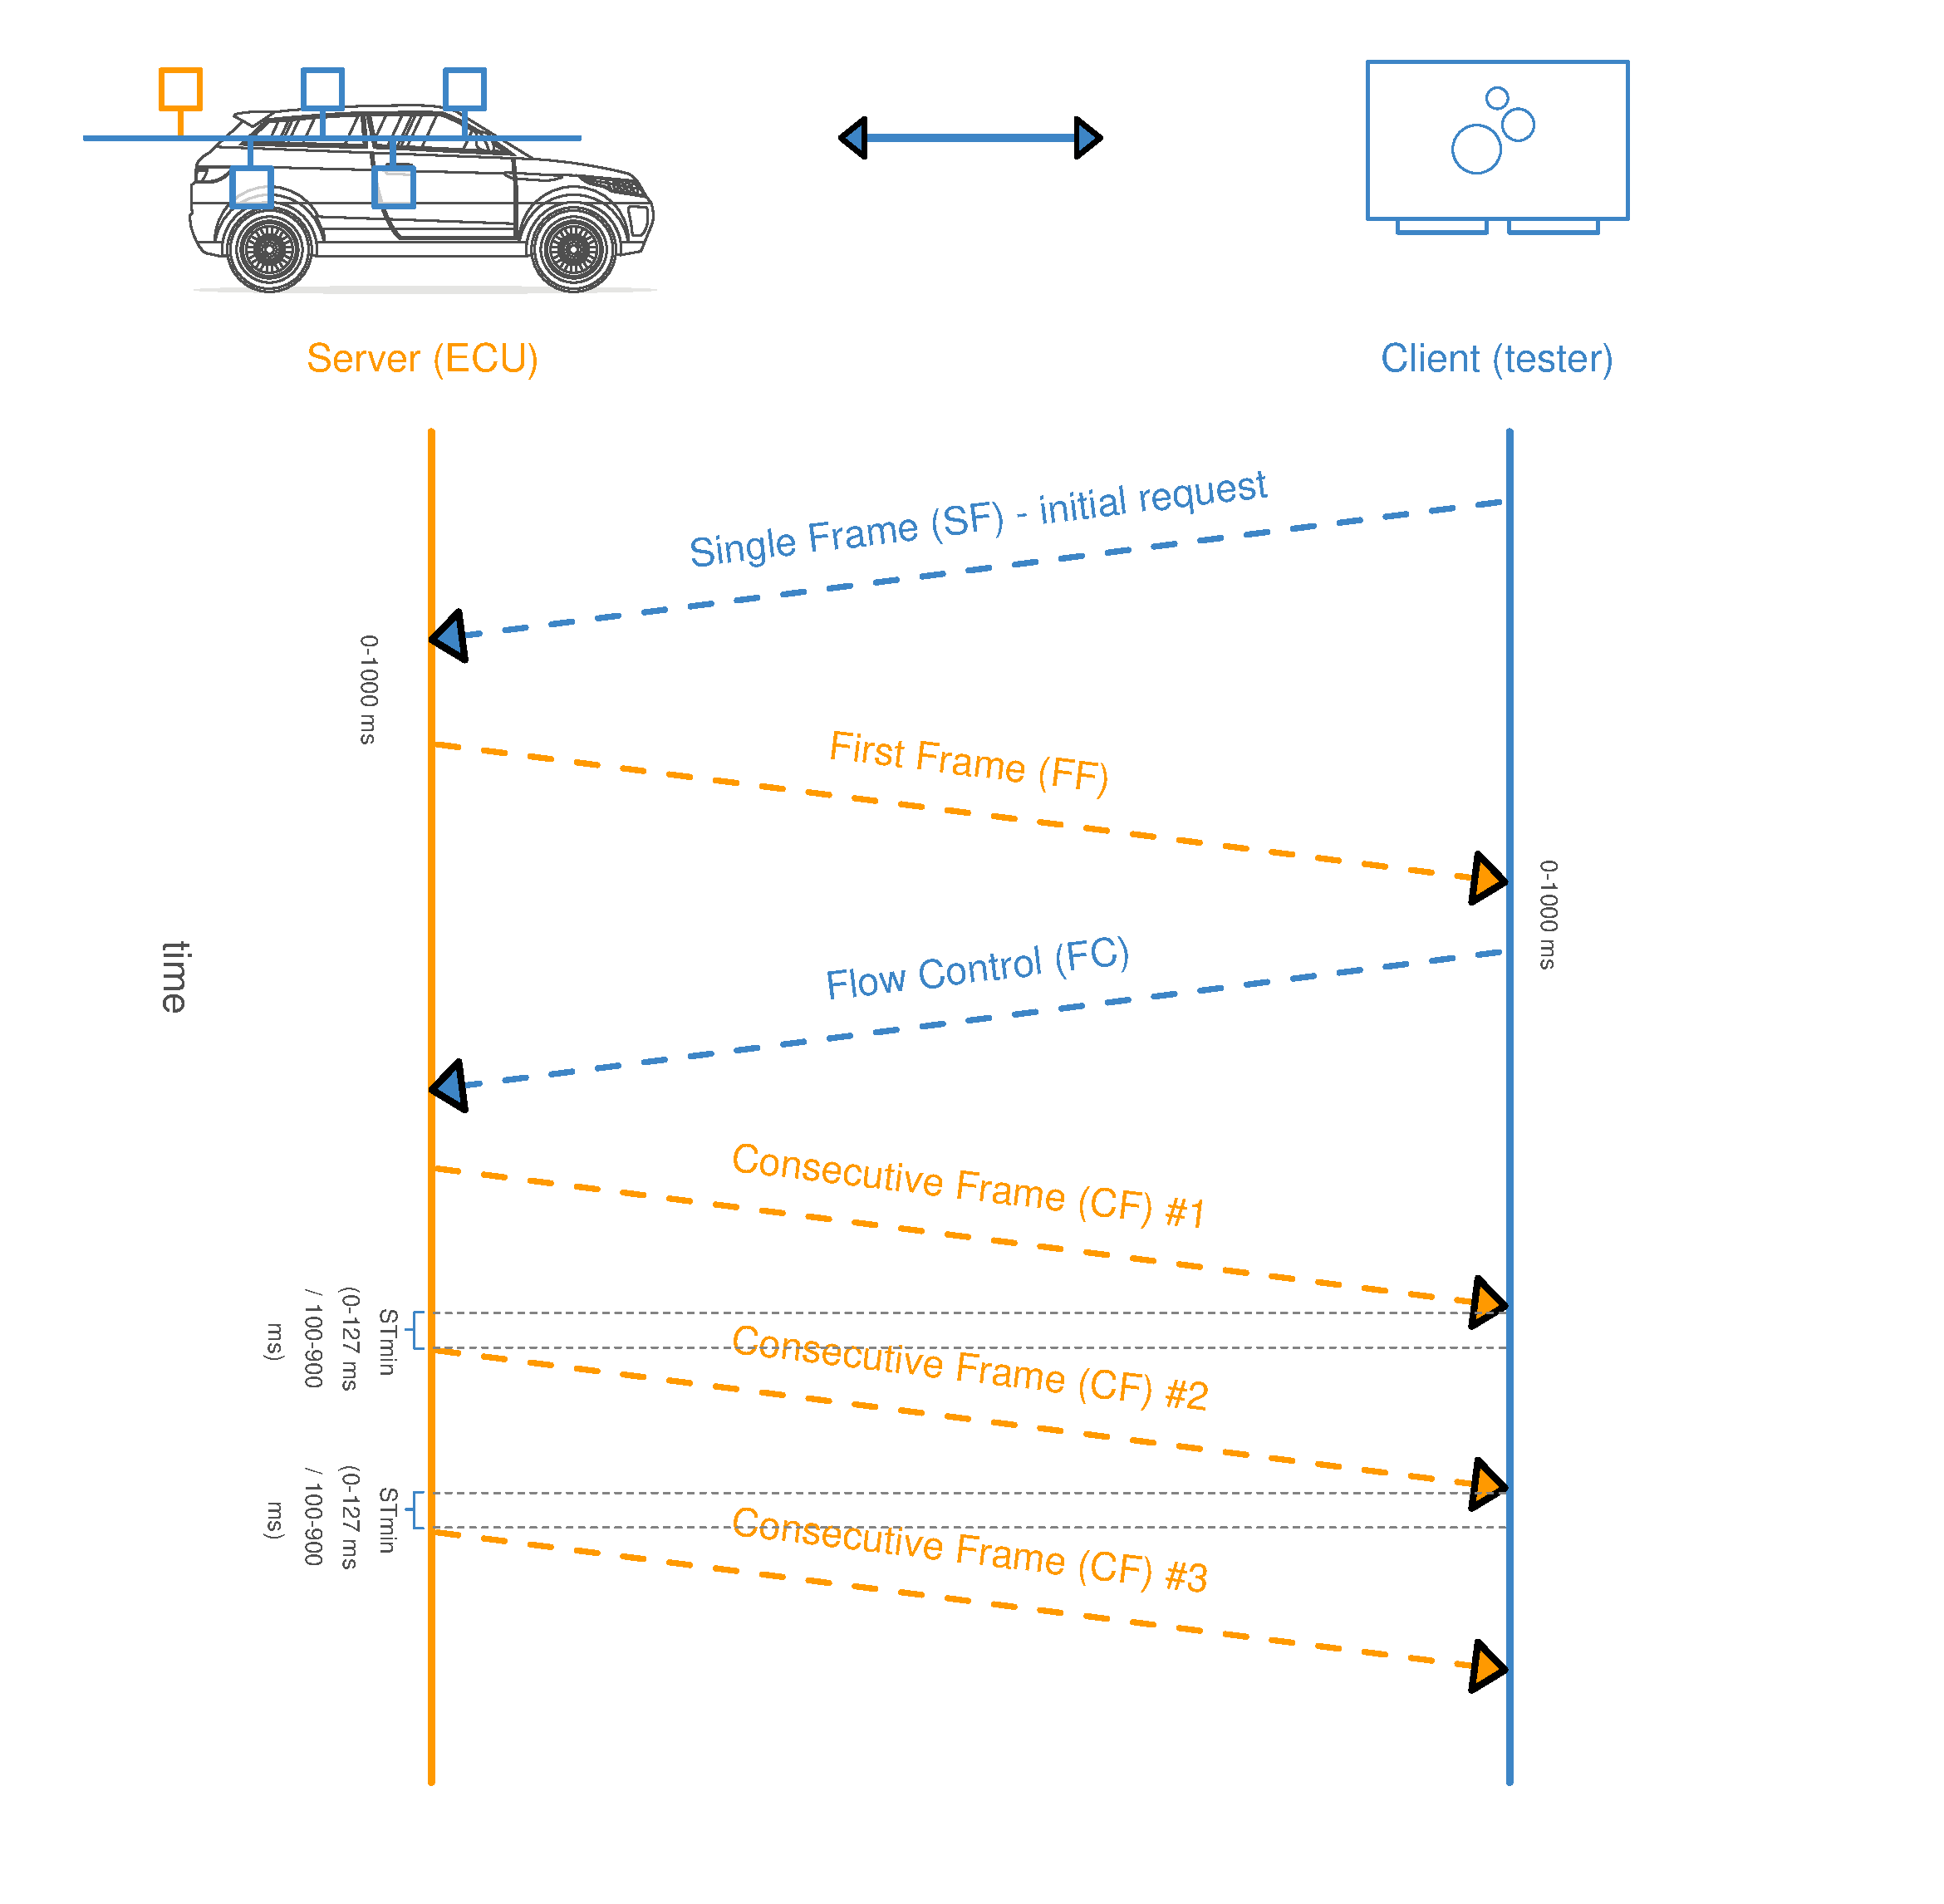
\includegraphics[width=0.78\textwidth]{implementation_uds_protocol.pdf}
\caption{ISO-TP message sequence between the tester (client) and the ECU (server) for a multi-frame UDS response: Single Frame request, First Frame, Flow Control, and Consecutive Frames separated by \texttt{STmin}.}
\label{fig:isotp_seq}
\end{figure}

\subsection{Unified Diagnostic Services (UDS)}
UDS, standardised in ISO 14229~\cite{iso14229}, is the \textbf{application-layer (OSI layer~7)} protocol used for all modern vehicle diagnostics, ECU programming and parameter reading. It sits at the very top of the diagnostic stack of Table~\ref{tab:osi_stack}: it defines \emph{what} is requested (services, sub-functions, Data Identifiers), while it deliberately says nothing about \emph{how} the bytes reach the ECU. The segmentation of long messages is delegated to ISO-TP one layer below (transport/network), and the actual bit transport to CAN at the data-link and physical layers. The same UDS service set therefore runs unchanged over CAN, CAN-FD, FlexRay, K-Line or DoIP/Ethernet -- only the lower layers differ. This layering is what makes UDS knowledge transferable: a service learned on one transport applies directly to any other, and the reverse-engineering strategy developed here would carry over to a future DoIP-based vehicle with the transport layer swapped out but the application dialogue intact.

Each UDS request is a byte stream starting with a one-byte Service Identifier (SID). The response either re-uses the SID increased by \hex{40} (positive response) or uses \hex{7F} followed by the original SID and an NRC (negative response code). For example, a read request with SID~\hex{22} is answered positively with SID~\hex{62}, or negatively with \hex{7F 22 \textit{NRC}} -- where the NRC \hex{31} means \textit{requestOutOfRange} (unknown DID/ECU) and \hex{33} means \textit{securityAccessDenied}. The negative response codes are informative in their own right during reverse engineering: a \hex{31} response tells the tester that the queried identifier is not implemented on that ECU and can be pruned from the search, whereas a \hex{33} response reveals that the identifier exists but lies behind a security-access barrier and would require a seed/key exchange to read. Distinguishing these two failure modes is what turns a blind sweep of candidate identifiers into a systematic mapping of what a given ECU exposes.

The services most relevant to this thesis are summarised in Table~\ref{tab:uds_services}. In particular, service \udssid{22} (\textit{ReadDataByIdentifier}) allows a tester to request the value of a specific two-byte Data Identifier (DID). ISO~14229-1~\cite{iso14229} partitions the 16-bit DID space into standardised and manufacturer-specific ranges; the largest vehicle-manufacturer-specific block is \hex{0100}--\hex{A5FF}, while \hex{F180}--\hex{F19F} holds standardised identification data and \hex{FF00}--\hex{FFFF} is reserved. All manufacturer-specific battery identifiers used in this work (for example \hex{028C}, \hex{1E3B}, \hex{1E40}, \hex{2A0B}, \hex{7448}) fall inside the \hex{0100}--\hex{A5FF} block, whereas \hex{F802} is an OBD-mapped identifier in the \hex{F800}--\hex{F8FF} range. Before such reads succeed, however, the tester usually has to raise the ECU out of its default session with \hex{10} (\textit{DiagnosticSessionControl}) into an extended session, and then keep that session alive with periodic \hex{3E} (\textit{TesterPresent}) messages, since an idle session times out and falls back to default after a few seconds. The interplay of these three services -- open the session, keep it alive, read the identifier -- forms the backbone of the acquisition procedure described in Section~\ref{sec:uds_procedure}.

\begin{table}[H]
\caption{UDS services relevant to the retrieval of battery data.}
\label{tab:uds_services}
\centering
\begin{tabular}{clp{7cm}}
\toprule
\textbf{SID} & \textbf{Service}             & \textbf{Purpose} \\
\midrule
\hex{10}     & DiagnosticSessionControl    & Switch between default, programming or extended session. \\
\hex{22}     & ReadDataByIdentifier        & Read the value stored under a 16-bit DID. \\
\hex{27}     & SecurityAccess              & Unlock protected data ranges via seed/key. \\
\hex{2E}     & WriteDataByIdentifier       & Write a value under a DID (not used here). \\
\hex{3E}     & TesterPresent               & Keep an extended session alive. \\
\bottomrule
\end{tabular}
\end{table}

\subsection{Diagnostic Addressing for Battery Data}
\label{ssec:diag_addr}
For a VW~Group vehicle built on the MEB platform, the battery management ECU (``HV battery'', BMS) answers on its own diagnostic CAN ID pair using 29-bit extended addressing. On the ID.~Buzz examined here the BMS is reached with request ID \hex{17FC007B} and replies on \hex{17FE007B}. This request/reply pairing is an instance of \emph{physical} (point-to-point) addressing: a request is directed at exactly one ECU, which answers on a fixed, closely related reply identifier, so that the tester can associate each response unambiguously with the ECU it queried. Other ECUs follow the same \hex{17FC00xx}/\hex{17FE00xx} scheme (e.g.\ DC/DC converter \hex{17FC00B9}/\hex{17FE00B9}, front EDU \hex{17FC0076}/\hex{17FE0076}), while a few comfort/gateway ECUs answer on classic 11-bit pairs (e.g.\ climate \hex{746}/\hex{7B0}, gateway \hex{710}/\hex{77A}). The regularity of the extended-identifier scheme, in which the low byte selects the target ECU, is itself a useful piece of reverse-engineering knowledge, because it lets a newly discovered ECU be addressed by analogy once the pattern is known.

A functional request to \hex{7DF} (the OBD-II broadcast request ID) reaches all emission-relevant ECUs simultaneously and is the starting point for any tester that does not yet know the physical addressing. In contrast to physical addressing, this \emph{functional} form is a one-to-many broadcast: every ECU that implements the requested service may answer, so the tester can discover which ECUs are present and which services they support before committing to a specific physical address. In practice a diagnostic session therefore often begins functionally, to enumerate the responders, and then continues physically, to interrogate a chosen ECU -- here the battery management controller -- in detail.

\section{The Volkswagen MEB Platform}
The Modular Electric Drive Matrix (\textit{Modularer E-Antriebs-Baukasten}, MEB) is Volkswagen Group's dedicated BEV platform, first used in production on the ID.3 in 2019. Unlike earlier electric vehicles that were adapted from combustion-engine platforms, the MEB was designed from the ground up around the battery and electric drivetrain, which allows a more efficient use of space and a network architecture tailored to the needs of an electric vehicle rather than retrofitted onto a legacy design. All ID-series vehicles -- including the ID.~Buzz used in this thesis -- share the same underlying architecture: a modular skateboard chassis with a flat battery pack between the axles, a rear-mounted permanent-magnet synchronous motor (single-motor variants) or an additional asynchronous motor on the front axle (4Motion variants), and a fully redesigned in-vehicle electrical and electronic architecture. Because the platform is shared across the whole ID family, insight gained on one MEB vehicle -- including the diagnostic addressing and the identifier layouts studied here -- is expected to transfer, at least in part, to its siblings.

From an electronic networking point of view, the MEB is organised around a small number of domain controllers (drive, chassis, comfort, infotainment, charging) connected to a central gateway ECU. Grouping functions into domains reduces the number of buses that must be interconnected and concentrates cross-domain routing in a single, well-defined place. The gateway isolates the private manufacturer CAN buses from the OBD-II connector; external testers see either the OBD-II emission CAN bus directly or -- in extended diagnostic sessions -- a subset of the internal buses routed through the gateway by UDS. This isolation is a deliberate design choice with both a safety and a security rationale: it prevents an external device from injecting arbitrary traffic onto the powertrain and battery buses, and it hides the internal broadcast messages -- including the raw battery frames -- from anything plugged into the diagnostic port. It is exactly this property that rules out a purely passive, byte-level recording of the battery traffic at the OBD-II connector and that makes the active, UDS-based approach of this thesis necessary.

The traction battery of the ID.~Buzz (Pro variant) has a gross capacity of 82~kWh (77~kWh net) at a nominal pack voltage of around 400~V. It is managed by a dedicated Battery Management Controller (BMC) and a series of cell-supervision circuits (CSC) that continuously report cell voltages and temperatures to the BMC over an internal battery CAN. This internal battery CAN is one of the private buses that the gateway keeps separate from the diagnostic port, so the detailed cell data it carries is not visible from the outside as ordinary broadcast traffic; it becomes reachable only when the BMC is addressed directly through the diagnostic services described above.

\section{High-Voltage Battery Systems in BEVs}
The lithium-ion pack of a modern BEV is not simply a larger version of a 12~V starter battery. It is an active system composed of several hundred individual cells, grouped into modules, managed by a dedicated electronic hierarchy. Where a starter battery is a passive energy store that is charged and discharged within a narrow band and largely ignored by the rest of the vehicle, a traction pack must be continuously supervised at the level of the individual cell, because both the safety and the usable lifetime of the pack depend on keeping every cell within tight voltage and temperature limits. The remainder of this section introduces the physical structure of the pack, the duties of the electronics that manage it, and the specific quantities this thesis sets out to observe.

\subsection{Cell, Module and Pack}
A single Li-ion cell has a nominal voltage of 3.6--3.7~V. In the ID.~Buzz, cells are connected in series to reach the pack nominal voltage, and in parallel to reach the desired capacity. The cells are organised into modules; each module has its own cell-supervision circuit that measures individual cell voltages (one measurement per cell) and one or more module temperatures. This three-level hierarchy -- cell, module, pack -- is what allows the management electronics to reason about the pack at the right granularity: safety decisions such as opening the contactors depend on the extreme values across all cells, whereas balancing and diagnostics depend on the value of each cell individually. Because the series connection means the weakest cell limits the whole string, per-cell measurement is not a luxury but a requirement, and it is the reason the pack exposes a long list of individual cell-voltage identifiers rather than a single aggregate figure.

\subsection{Battery Management System}
The Battery Management System (BMS) is responsible for keeping the pack within its safe operating area. It continuously compares the measured cell voltages, temperatures and currents against the limits defined for the chemistry, and it intervenes -- by limiting power, requesting cooling or heating, or ultimately opening the contactors -- whenever a limit is approached, so that the pack is protected against overcharge, deep discharge, over-current and thermal runaway. Its core duties are:

\begin{itemize}
  \item monitoring every cell voltage and every module temperature;
  \item estimating the pack state of charge (SOC) and state of health (SOH);
  \item controlling the main positive and negative contactors;
  \item performing cell balancing (passive or active) during charging;
  \item reporting power limits (charge/discharge) to the inverter and the charger.
\end{itemize}

Each of these duties leaves an observable trace in the data the BMS holds internally, and it is this internal state that the diagnostic queries of this thesis aim to read out. The monitoring duty produces the per-cell voltage and per-point temperature values; the estimation duty produces the SOC and SOH figures shown on the dashboard; the contactor and power-limit duties determine the operating mode the pack reports. Reconstructing the meaning of the corresponding data identifiers is therefore, in effect, reconstructing a view of the BMS's own working picture of the pack.

SOC in particular is not a directly measurable quantity. It is estimated by the BMS from a combination of coulomb counting, open-circuit-voltage look-ups and model-based filters such as Kalman filters. Coulomb counting integrates the measured current over time to track how much charge has entered or left the pack, but it accumulates drift and must be periodically corrected; the open-circuit voltage of a cell at rest gives an independent, if slow, anchor for the true state of charge; and a model-based filter fuses these sources while accounting for their respective uncertainties. The estimate that the BMS reports to the driver's dashboard is therefore a conservative, smoothed version of a much richer internal state. This indirection matters for the validation strategy of this thesis: because the reported SOC is a filtered estimate rather than a raw sensor reading, agreement between a decoded identifier and the dashboard value confirms not only that the byte layout and scaling are correct but also that the identifier being read is indeed the one the BMS presents to the driver.

\subsection{Signals of Interest}
For this thesis, the following battery parameters are considered the primary targets. They were chosen because together they span the safety-critical and the informational aspects of the pack: the aggregate quantities (state of charge, terminal voltage, current, state of health) describe the pack as a whole, while the per-cell extremes (minimum and maximum cell voltage and temperature) describe its internal spread and therefore its health and safety margin. Recovering these quantities, and confirming their scaling against the physical vehicle, is the concrete objective around which the acquisition and decoding chapters are built.

\begin{table}[H]
\caption{Battery parameters targeted by the UDS queries in this thesis.}
\label{tab:battery_signals}
\centering
\begin{tabular}{lp{4cm}l}
\toprule
\textbf{Parameter}           & \textbf{Typical scale}             & \textbf{Expected DID range} \\
\midrule
Pack state of charge         & 0--100\,\%, 0.5\,\% resolution     & manufacturer-specific \\
Pack terminal voltage        & 0--500\,V, 0.1\,V resolution       & manufacturer-specific \\
Pack current                 & $\pm$500\,A, signed, 0.1\,A res.   & manufacturer-specific \\
Cell voltage min / max       & 2.5--4.25\,V, 1\,mV resolution     & manufacturer-specific \\
Cell temperature min / max   & $-40$\,\textdegree{}C--+80\,\textdegree{}C & manufacturer-specific \\
State of health              & 0--100\,\%                         & manufacturer-specific \\
\bottomrule
\end{tabular}
\end{table}

\section{State of the Art of CAN Bus Reverse Engineering}
\label{sec:sota}
The systematic reverse engineering of automotive CAN networks has been pursued in both the research and the open-source communities, motivated by the fact that the mapping from raw bus traffic to physical signals is almost never published by vehicle manufacturers. Two lines of prior work bear on the present thesis: the community-maintained effort to collect and share signal databases across many vehicles, and the academic work on recovering signal encodings from recorded traffic.

On the open-source side, the \texttt{opendbc}~\cite{opendbc} repository maintained by comma.ai collects community-contributed CAN signal descriptions for a large number of vehicles. It is the best-known example of the community database effort, and it illustrates both the value and the limits of that model: coverage is broad but uneven, entries are contributed without a formal validation procedure, and what is documented reflects what contributors happened to need. It should be stated clearly that \texttt{opendbc} is \emph{not} a source for this work and could not be. It describes \emph{broadcast} CAN signals in DBC form; it contains no UDS Data Identifiers and does not document Volkswagen's \hex{17FC00xx}/\hex{17FE00xx} diagnostic addressing, so none of the identifiers used here can be cross-checked against it.

The artefact this thesis actually builds on belongs to the same tradition but is a different document: a publicly circulating identifier list for the VW~ID.3~\cite{vwmebpidlist}, which supplies a target address, a request frame, a response layout and a decoding equation for 161~manufacturer-specific identifiers. Its author reports testing on VW~ID.x and \v{S}koda Enyaq vehicles and expects broader MEB compatibility, while naming the differing battery cell count between models as the principal parameter that must be adapted per car -- an open question that Section~\ref{ssec:cellcount} answers for the ID.~Buzz. Like \texttt{opendbc}, the list carries no licence, no authorship trail and no validation record, and it was compiled for a different vehicle than the one studied here. It is therefore treated throughout this work as a hypothesis to be tested rather than a reference to be trusted, and testing it is a substantial part of what Chapter~4 reports.

The academic literature on CAN reverse engineering is almost exclusively concerned with the \emph{passive} problem: given a recording of broadcast traffic, recover the signal boundaries and encodings without documentation. Marchetti and Stabili's READ~\cite{read} locates candidate signal boundaries from the bit-flip rates of successive frames, exploiting the fact that the low-order bits of a physical quantity toggle far more often than its high-order bits. LibreCAN~\cite{librecan} extends this into a pipeline that correlates candidate signals against an external ground truth -- smartphone inertial data and standard OBD-II PIDs -- to attach physical meaning automatically. CAN-D~\cite{cand} formalises the same task as a four-step pipeline covering tokenisation, endianness, signedness and scaling. Huybrechts et al.~\cite{huybrechts2018automatic} approach the boundary problem with machine learning, comparing an arithmetic method against a classifier.

All four share the precondition this thesis cannot satisfy: they require the target ECU's broadcast frames to be observable. The evidence of Section~\ref{ssec:broadcast} is that the battery frames are not present at the diagnostic connector of the ID.~Buzz, and none of these techniques has anything to operate on there. No academic study was found that reverse engineers battery data from an MEB-platform vehicle, or that addresses the case in which the target frames are gated behind a domain gateway and only the diagnostic channel remains. The closest relevant body of knowledge is not academic at all but the community identifier list~\cite{vwmebpidlist} on which this work builds, and that artefact is undocumented, unvalidated and compiled for a different vehicle. Establishing whether it transfers is precisely the gap this thesis addresses.

% ============================================================

% ============================================================
\chapter{Materials and Methods}
% ============================================================
This chapter explains the selection of the test vehicle, the preparation of the measurement hardware, the experimental setup and the software tool chain used to record and analyse the CAN data. The order of presentation deliberately follows the physical signal path: from the vehicle that produces the battery data, through the logger that both stimulates and records the diagnostic bus, to the offline software that converts the raw log into engineering quantities. Each stage is described together with the reasoning behind the design choice, because several of these choices -- in particular the use of a transmit-capable logger and the decision to interrogate the battery actively rather than to observe it passively -- are direct consequences of how the vehicle architecture exposes (and, more importantly, hides) the battery-management data. The reverse-engineering methodology and the concrete diagnostic procedure that build on this setup are then developed in the later sections of the chapter.

\section{Test Vehicle: Volkswagen ID.~Buzz}
All measurements were performed on THI's Volkswagen ID.~Buzz Pro (2024): 77~kWh net battery capacity, rear-wheel drive with a 150~kW permanent-magnet synchronous motor, running ID.~Software~4.x. The sessions analysed in Chapter~4 were recorded with the pack at 72--73\,\% SOC, comfortably inside the normal working band and well clear of the low-SOC region in which the battery-management system progressively derates available power.

\begin{figure}[H]
\centering
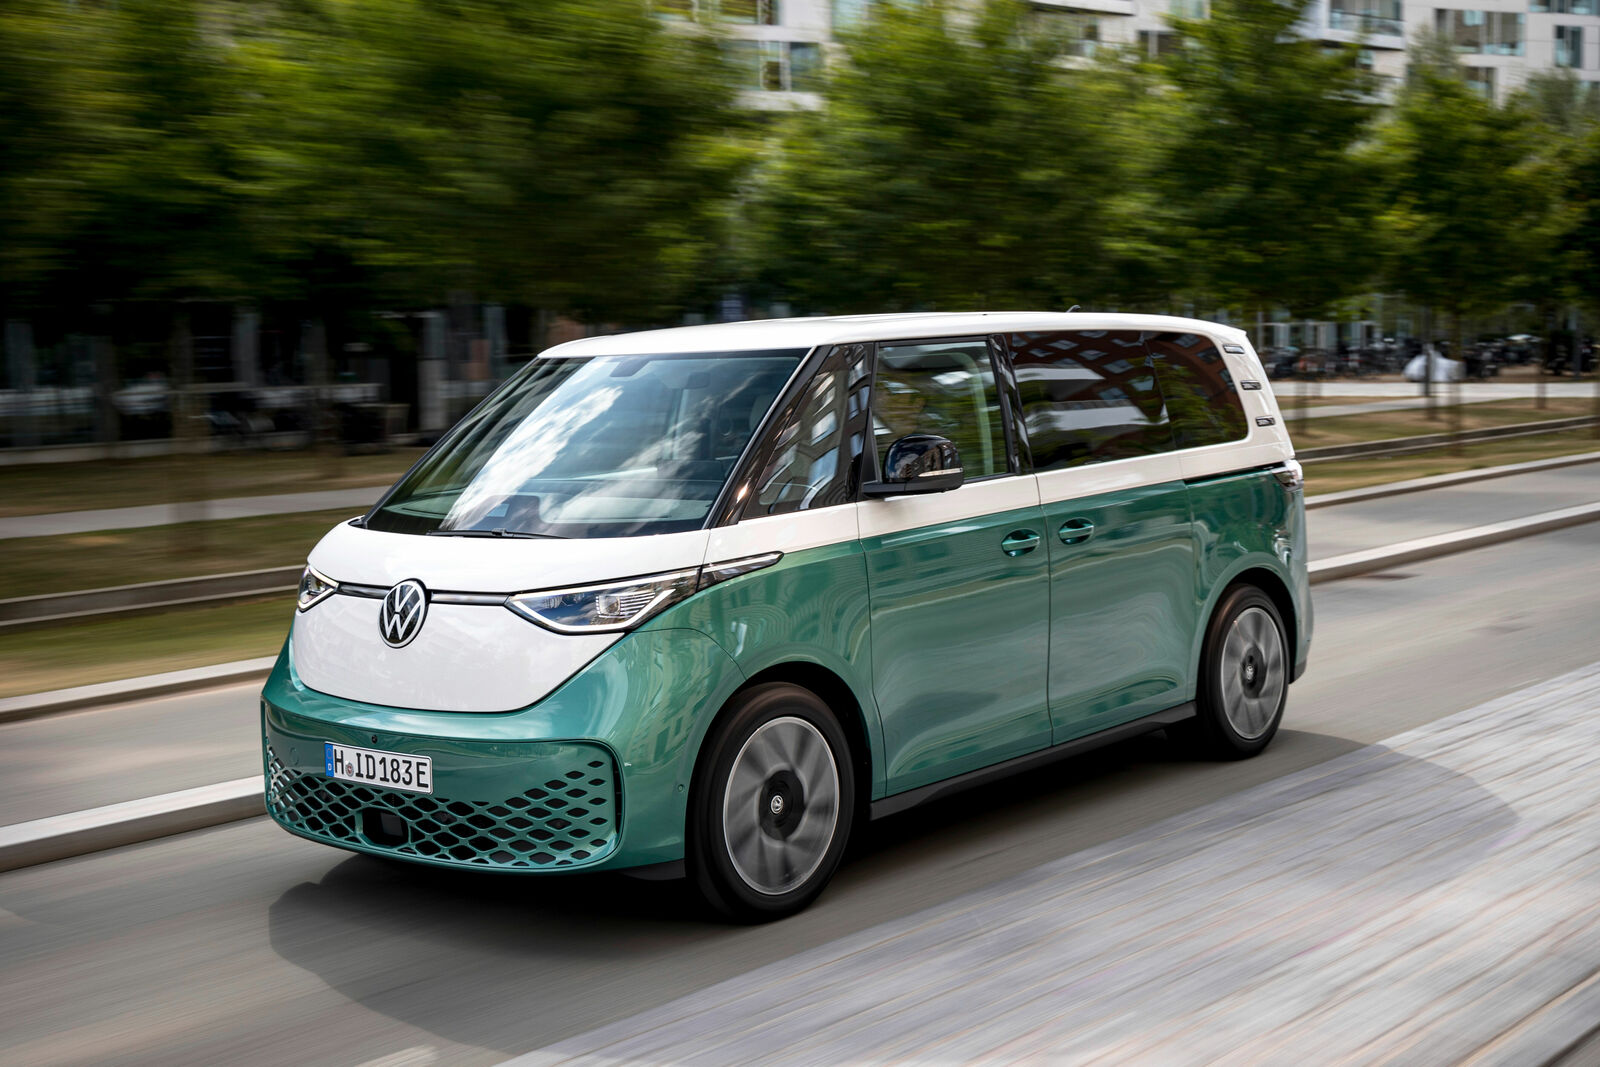
\includegraphics[width=0.85\textwidth]{id_buzz.jpg}
\caption[The test vehicle]{The Volkswagen ID.~Buzz (manufacturer image). All measurements in this thesis were made on THI's vehicle of this type, through its OBD-II connector and with the vehicle stationary.}
\label{fig:idbuzz}
\end{figure}

The vehicle is not an incidental choice. The Modular Electric Drive Matrix (\textit{Modularer E-Antriebs-Baukasten}, MEB) underpins a large family of production vehicles sharing the same high-voltage architecture, battery-management electronics and diagnostic addressing, so findings obtained here transfer at least structurally to siblings such as the ID.3 and ID.4. Being a recent series-production car, it also carries the full production security posture of the platform -- including the gateway isolation of Section~\ref{sec:why_uds} -- so the constraints met here are the real ones a workshop or researcher would face, not artefacts of a prototype. The 77~kWh net pack (82~kWh gross) runs at roughly 400~V nominal and is built from pouch cells grouped into modules and connected as a series string of parallel cell groups. The number of \emph{series} groups sets the pack voltage and equals the number of cell voltages the management system measures; it is not published at the detail needed here, and Section~\ref{ssec:cellcount} establishes it from the measurements as~96. The identifier block reserves more cell slots than the pack populates, so its size must not be mistaken for the physical cell count.

\begin{figure}[H]
\centering
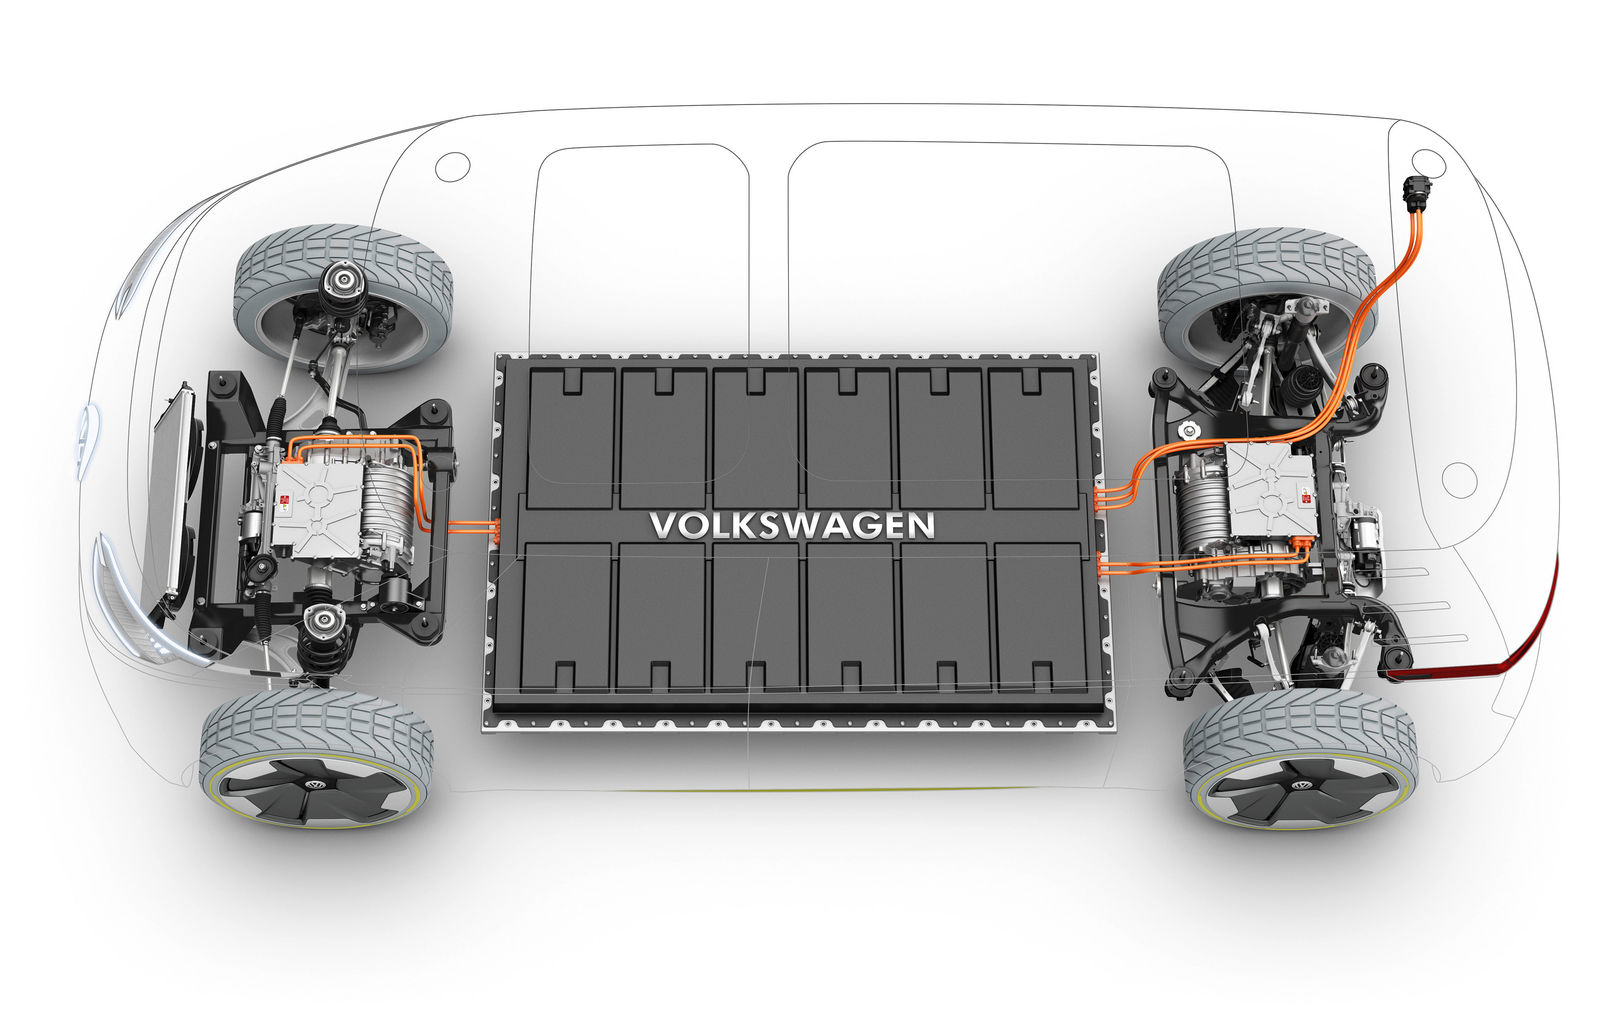
\includegraphics[width=0.9\textwidth]{id_buzz_system.jpg}
\caption[High-voltage system of the ID.~Buzz]{Simplified overview of the high-voltage system of the ID.~Buzz: the traction battery with its battery-management system, the power electronics and the drive unit. The battery-management system is the control unit interrogated over UDS in this work.}
\label{fig:idbuzz_system}
\end{figure}

\section{Hardware Setup}
\subsection{CANedge2 Data Logger}
The CAN frames were recorded with a CANedge2 data logger (CSS Electronics)~\cite{csselectronics_canedge2}. This device has two independent CAN channels, each with a 24-bit hardware timestamp, supports CAN Classical and CAN-FD, and stores data on an SD card in the ASAM~MDF~4.11 format~\cite{asammdf}. Its power is drawn from pin~16 (battery~+) of the OBD-II connector, which means the logger stays active as long as the vehicle has power -- including the short wake-up interval after the vehicle is unlocked. Channel~1 was configured for Classical CAN at 500~kbit/s; channel~2 was left in listen-only mode for an optional second tap.

The hardware timestamp deserves emphasis, because the entire later analysis relies on being able to associate each response with the request that provoked it. A 24-bit timestamp generated in the logger's own hardware, rather than assigned in software after the fact, means that every frame -- transmitted or received -- carries a precise and monotonic time reference from a single clock. When requests and responses are written into the same file with the same time base, matching a positive UDS answer to its originating ReadDataByIdentifier request becomes a straightforward temporal-proximity problem instead of a fragile reconstruction. The 500~kbit/s Classical CAN configuration on channel~1 matches the physical characteristics of the OBD-II diagnostic bus of the ID.~Buzz, which is a Classical CAN bus and not CAN-FD~\cite{iso11898}; configuring the channel to the exact bus bit rate is a precondition for the controller to acknowledge frames and participate on the bus at all. Channel~2 was held in listen-only mode as an optional second tap, so that an additional bus could be observed without any risk of the logger disturbing it.

\begin{figure}[H]
\centering
\begin{subfigure}[b]{0.49\textwidth}
  \centering
  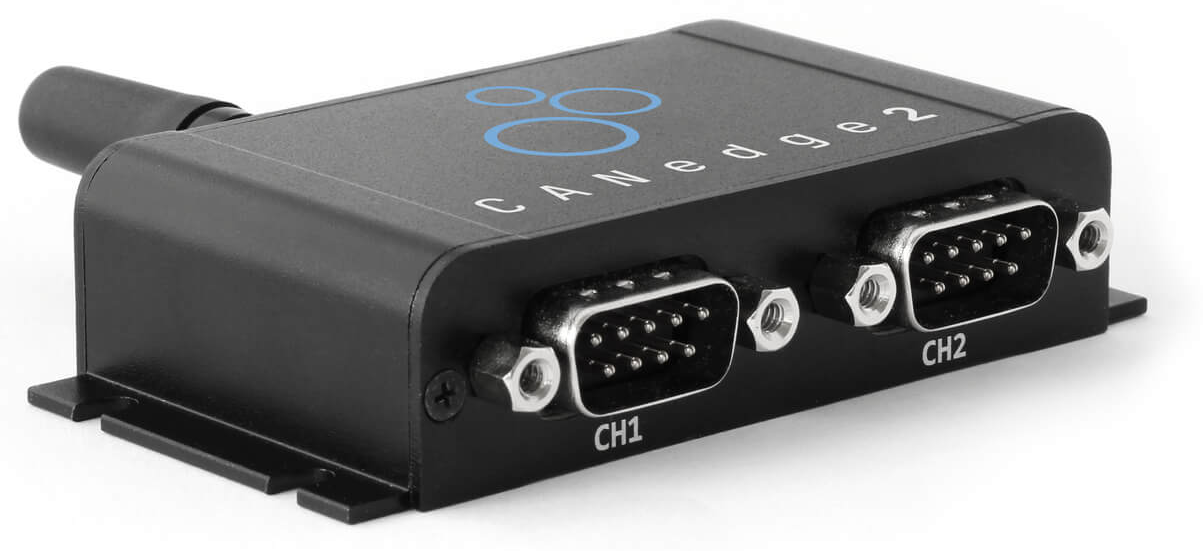
\includegraphics[width=\linewidth]{canedge2_front_big.png}
  \caption{Front view: the two DB9 connectors CH1 and CH2.}
  \label{fig:canedge_front}
\end{subfigure}
\hfill
\begin{subfigure}[b]{0.49\textwidth}
  \centering
  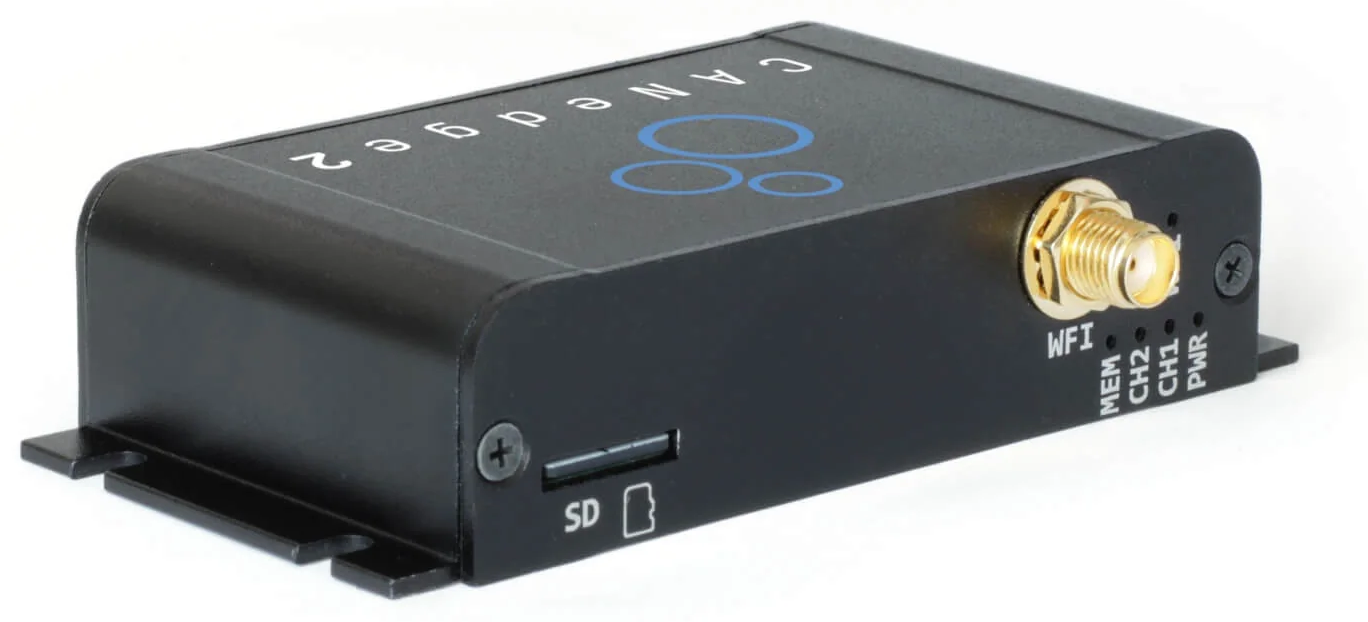
\includegraphics[width=\linewidth]{canedge2_back_big.png}
  \caption{Rear view with the SD-card slot.}
  \label{fig:canedge_back}
\end{subfigure}
\caption{The CANedge2 data logger (CSS Electronics) used in this thesis. CH1 is connected to the OBD-II HS-CAN bus of the ID.~Buzz; CH2 is left in listen-only mode.}
\label{fig:canedge2}
\end{figure}

Crucially, the CANedge2 is not only a passive logger: each CAN channel has a configurable \textit{transmit list} that can periodically send up to 64 user-defined CAN frames onto the bus and log the responses in the same MF4 file. In this thesis that transmit list is used to issue the UDS requests directly from the logger, so that \textbf{the active UDS retrieval of battery data is performed by the CANedge2 itself} rather than by a separate diagnostic tester. This makes the active and passive data appear in one synchronised, hardware-timestamped recording. The device used here runs firmware~01.08.01 with configuration schema~01.08.

The transmit capability is the single most important reason the CANedge2 was chosen over a purely passive logger, because the battery data on this platform cannot be recovered by listening alone (Section~\ref{sec:why_uds}); it must be elicited by sending diagnostic requests. A conventional logger would force the setup to include a second, separately clocked device -- a dedicated diagnostic tester -- to generate those requests, after which the requests and the responses would live in two files with two time bases that must be aligned in post-processing. By collapsing the stimulus and the recording into one device, the transmit list eliminates that alignment problem entirely and guarantees that every logged response is timestamped on the same clock as the request that caused it. The consequence of this design choice, both its benefits and its one significant limitation, runs through the whole of the diagnostic procedure described in Section~\ref{sec:uds_procedure}.

\subsection{OBD-II Connection}
The CANedge2 was connected directly to the vehicle's OBD-II socket with a standard OBD-II--to--DB9 adapter cable on channel~1; no Y-splitter or parallel tester was used. The cable carries the CAN-H, CAN-L, ground and battery-positive lines on pins~6, 14, 4/5 and 16 respectively (compare Table~\ref{tab:obd2_pins}), so the logger is both powered and bus-connected through the single OBD-II connector.

\begin{figure}[H]
\centering
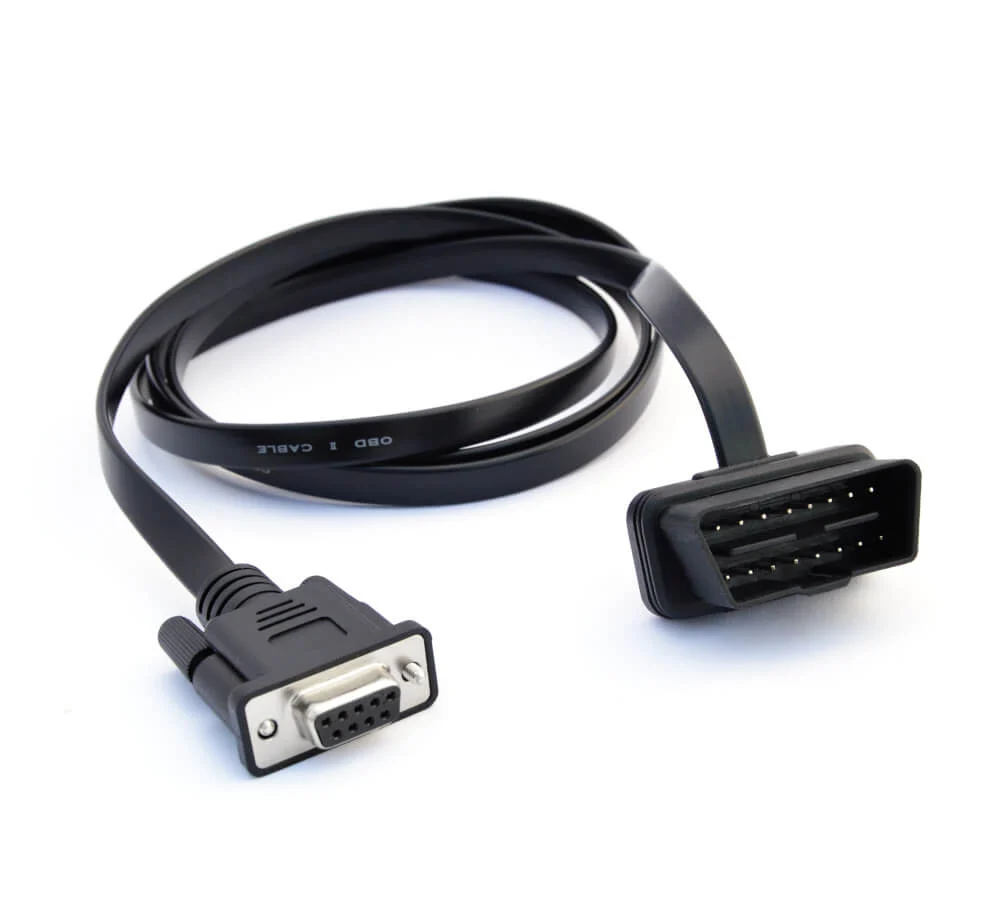
\includegraphics[width=0.6\textwidth]{obd2_db9_cable.png}
\caption[OBD-II--to--DB9 adapter cable]{The OBD-II--to--DB9 adapter cable used to connect channel~1 of the CANedge2 to the diagnostic connector of the ID.~Buzz. It carries CAN-H, CAN-L, ground and battery-positive from the OBD-II pins listed in Table~\ref{tab:obd2_pins} to the DB9 connector of the logger.}
\label{fig:obd2_cable}
\end{figure}

The decision to use a single, direct connection rather than a Y-splitter feeding both the logger and a workshop tester in parallel is deliberate and has a clear technical justification. The OBD-II connector and its pin assignment are standardised~\cite{saej1962}, so a direct adapter reliably exposes the high-speed CAN pair together with ground and switched battery power on the pins listed above. Adding a second active device on the same bus through a splitter would introduce another node that arbitrates for the bus, acknowledges frames and potentially issues its own diagnostic traffic. On a diagnostic bus that traffic could collide or interleave with the requests emitted by the transmit list, could open or reset diagnostic sessions on the very ECUs under study, and would in any case make it impossible to attribute observed responses unambiguously to the logger's own requests. Keeping the CANedge2 as the sole diagnostic node on the bus removes these confounders, so that every request on the bus is one the logger sent and every response can be traced back to it. Drawing both power and bus connection through the single OBD-II connector also keeps the physical setup minimal and repeatable, which matters for a measurement that is rotated across several sessions and configurations.

\begin{figure}[H]
\centering
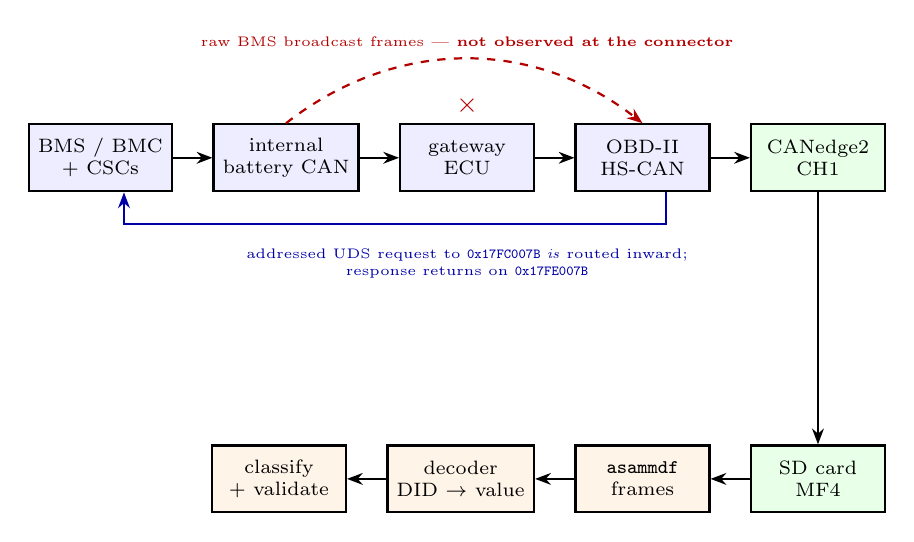
\begin{tikzpicture}[
  font=\scriptsize,
  blk/.style={draw,thick,minimum height=8.5mm,minimum width=17mm,align=center},
  veh/.style={blk,fill=blue!7},
  log/.style={blk,fill=green!9},
  pcs/.style={blk,fill=orange!9},
  ar/.style={-{Stealth[length=2mm]},thick}]

\node[veh] (bms)  {BMS / BMC\\+ CSCs};
\node[veh,right=5mm of bms]  (ibus) {internal\\battery CAN};
\node[veh,right=5mm of ibus] (gw)   {gateway\\ECU};
\node[veh,right=5mm of gw]   (obd)  {OBD-II\\HS-CAN};
\node[log,right=5mm of obd]  (ce)   {CANedge2\\CH1};

\node[log,below=32mm of ce]  (sd)   {SD card\\MF4};
\node[pcs,left=5mm of sd]    (asam) {\texttt{asammdf}\\frames};
\node[pcs,left=5mm of asam]  (dec)  {decoder\\DID $\to$ value};
\node[pcs,left=5mm of dec]   (val)  {classify\\+ validate};

\foreach \a/\b in {bms/ibus, ibus/gw, gw/obd, obd/ce} \draw[ar] (\a) -- (\b);
\draw[ar] (ce) -- (sd);
\foreach \a/\b in {sd/asam, asam/dec, dec/val} \draw[ar] (\a) -- (\b);

% blocked broadcast path (above row 1); flat arc so the label clears it
\draw[ar,dashed,red!70!black] (ibus.north) to[out=38,in=142] (obd.north);
\node[red!70!black,font=\bfseries] at ([yshift=2.2mm]gw.north) {$\times$};
\node[align=center,font=\tiny,red!70!black,above=8.5mm of gw.north]
   {raw BMS broadcast frames --- \textbf{not observed at the connector}};

% routed diagnostic path (rectangular, in the gap below row 1)
\draw[ar,blue!65!black]
   ([xshift=3mm]obd.south) -- ([xshift=3mm,yshift=-4mm]obd.south)
   -- ([xshift=3mm,yshift=-4mm]bms.south) -- ([xshift=3mm]bms.south);
\node[align=center,font=\tiny,blue!65!black,below=6mm of gw.south]
   {addressed UDS request to \hex{17FC007B} \emph{is} routed inward;\\response returns on \hex{17FE007B}};
\end{tikzpicture}
\caption[Signal path from cell to engineering value]{Signal path from the physical cell to the interpreted engineering value. The battery-management frames broadcast on the internal bus are not observed at the diagnostic connector (red, Section~\ref{ssec:broadcast}), but addressed diagnostic requests are routed inward and their responses returned (blue). The CANedge2 is powered from pin~16 of the same connector and writes MDF4 files to its SD card for offline analysis.}
\label{fig:setup}
\end{figure}

\section{Software Tool Chain}
\label{sec:toolchain}
The recorded MDF4 files were processed entirely in Python~3.12. The actual conversion from the binary MF4 log into engineering data is performed by the \textbf{\texttt{asammdf}} library~\cite{asammdf}: it parses the ASAM~MDF~4.11 container, decodes the embedded CAN frame groups (arbitration ID, DLC, raw payload bytes and hardware timestamp) and exposes them as \texttt{numpy} arrays. A thin custom module, \texttt{mf4\_reader.py} (built on \texttt{asammdf} together with \texttt{numpy} and \texttt{pandas}), flattens each frame into a \texttt{pandas} DataFrame with the columns described in Table~\ref{tab:mf4_columns}; a companion converter (\texttt{mf4\_converter.py}) uses the same \texttt{asammdf} backend to export the raw frames to SavvyCAN-compatible CSV for cross-checking. The physical battery quantities are then obtained by applying the per-DID scaling formulas of the master PID list (Section~\ref{sec:uds_procedure}) to the decoded UDS response bytes.

Building the tool chain on top of \texttt{asammdf} rather than parsing the binary container by hand is a pragmatic choice: the MF4 container is a rich, standardised format with channel groups, conversion rules and metadata, and a mature library handles the low-level container details reliably so that the analysis code can work with clean \texttt{numpy} arrays. Flattening each frame into a uniform DataFrame, as defined in Table~\ref{tab:mf4_columns}, gives every later stage of the pipeline a single, predictable data structure to operate on, independent of which log or which session a frame came from. The parallel export to SavvyCAN-compatible CSV via \texttt{mf4\_converter.py} provides an independent way to inspect the same raw frames in an established CAN-analysis tool, which is valuable as a cross-check during reverse engineering: if a frame is misread in the custom pipeline, the discrepancy against the SavvyCAN view surfaces it immediately.

\begin{table}[H]
\caption{Normalised frame format used across the analysis pipeline.}
\label{tab:mf4_columns}
\centering
\begin{tabular}{lll}
\toprule
\textbf{Column} & \textbf{Type}       & \textbf{Description} \\
\midrule
timestamp       & float (index)      & Seconds from recording start. \\
can\_id         & int                & CAN arbitration ID; 11-bit for broadcast traffic, 29-bit for the diagnostic exchange. \\
can\_id\_hex    & string             & Hex representation, e.g.\ \texttt{0x065}. \\
dlc             & int                & Data-length code, 1--8. \\
data\_bytes     & byte array         & Raw payload. \\
data\_hex       & string             & Space-separated hex payload. \\
bus\_channel    & int                & Channel tag as written by the logger (values 1 and 9 occur). \\
direction       & int                & 0 = received, 1 = transmitted by the logger. \\
source          & string             & Source log folder identifier. \\
\bottomrule
\end{tabular}
\end{table}

On top of \texttt{mf4\_reader.py} the analysis pipeline comprises:

\begin{itemize}
  \item \texttt{can\_analyzer.py} -- enumerates the CAN IDs present in a log and counts the request/response frames, used to verify that each UDS request received an answer.
  \item \texttt{uds\_decoder.py} -- extracts the UDS response frames that the CANedge2 logged on the BMS reply ID \hex{17FE007B}, matches each one to its request, and decodes the Data Identifier payloads into physical battery parameters using the per-DID scaling formulas.
\end{itemize}

These two modules separate two distinct concerns. The \texttt{can\_analyzer.py} module operates at the level of the bus itself: by enumerating the arbitration IDs present in a log and counting request and response frames, it answers the bookkeeping question of whether the diagnostic exchange actually completed -- that is, whether each request that was transmitted was in fact answered. The \texttt{uds\_decoder.py} module operates one layer higher, at the level of the diagnostic protocol: it isolates the UDS responses that the BMS returned on its reply identifier \hex{17FE007B}, pairs each response with the request that elicited it, and applies the per-DID scaling formulas to turn the raw payload bytes into physical battery parameters. This layered structure mirrors the reverse-engineering methodology of Section~\ref{sec:re_methodology}: coverage and completeness are established first, and only the responses that are actually present are then interpreted and scaled.

\section{Why Active UDS Instead of Passive Reverse Engineering}
\label{sec:why_uds}
Classical CAN reverse engineering is \textit{passive}: the analyst taps the bus on which the target ECU broadcasts, records its frames and recovers the signal layout statistically. This was the originally planned approach for the BMS of the ID.~Buzz, but it is not feasible from the OBD-II connector. The BMS broadcasts its raw measurement frames only on the private internal battery/powertrain CAN bus. On the MEB platform a central gateway ECU separates these internal buses from the OBD-II diagnostic bus and, for security reasons, does not forward the raw BMS broadcast frames to the outside. The broadcast traffic that does reach the OBD-II port was examined and contains nothing attributable to the battery (Section~\ref{ssec:broadcast}), so a passive byte-level reverse engineering of the battery signals cannot be performed there without invasively tapping the high-voltage battery wiring -- which is out of scope and unsafe on a production vehicle.

The role of the gateway is central to understanding this constraint. In a modern vehicle the individual CAN buses are not one flat network; they are segmented into domains -- powertrain, chassis, comfort, infotainment and a dedicated diagnostic connection -- that are joined only through a central gateway ECU. The gateway acts as a controlled boundary: it decides which messages cross from one domain to another and which do not. The private battery and powertrain bus, on which the BMS continuously broadcasts its cyclic measurement frames, sits behind this boundary. From a security and robustness standpoint there is no reason for the manufacturer to relay those internal broadcast frames to the externally accessible OBD-II bus, and on the MEB platform they are not relayed. A passive tap on the OBD-II connector therefore sees the diagnostic traffic and whatever else the gateway chooses to expose. What it does expose is not nothing: the recordings of this work contain 14\,921 unsolicited broadcast frames on six standard identifiers, and Section~\ref{ssec:broadcast} examines them. None of them could be attributed to the battery. This is the precondition that the passive reverse-engineering literature~\cite{read,librecan,cand,huybrechts2018automatic} assumes and that is absent here: those methods recover signal boundaries from broadcast traffic, and at this measurement point the battery's broadcast traffic is not available to recover anything from.

What the gateway \emph{does} forward are addressed UDS diagnostic requests. The BMS answers these on its diagnostic reply ID, so the battery data is reachable actively even though it is not reachable passively. The work therefore proceeds entirely via UDS.

The reason the gateway forwards diagnostic requests is functional: legitimate servicing, workshop diagnosis and regulatory readiness checks all depend on an external tester being able to address individual ECUs through the OBD-II connector and receive their answers. The gateway routes such addressed requests to the correct internal ECU and returns the response, because that is exactly what the diagnostic architecture exists to support. This is what turns an otherwise inaccessible dataset into an accessible one: rather than waiting for the BMS to volunteer its state on a bus that never reaches the connector, the setup asks the BMS directly, on the diagnostic channel the gateway is designed to relay. The remainder of the chapter therefore concentrates on how those requests are constructed, addressed and interpreted.

\section{Reverse-Engineering Methodology}
\label{sec:re_methodology}
Volkswagen publishes neither the manufacturer-specific Data Identifiers of the battery controller nor their encodings. The ID.3 branch of the MEB platform has, however, been characterised by the independent diagnostics community, and a publicly circulating identifier list for the VW~ID.3~\cite{vwmebpidlist} proposes, for each of 161~identifiers, a target ECU address, a request frame, a response layout and a linear decoding equation. It is essential to be precise about the status of this artefact, because the integrity of every number in Chapter~4 depends on it. The list states no author, no licence and no validation procedure; its column structure is built around the \texttt{ATSH} and \texttt{ATCRA} commands of the ELM327 OBD adapter, which indicates that it originated from dongle-based experimentation rather than from manufacturer documentation; and it was compiled for the ID.3, not for the ID.~Buzz. It is therefore treated throughout this work as a \textbf{hypothesis to be tested, not as a specification to be trusted}, and every equation reproduced in Chapter~4 is attributed to it.

This defines the reverse-engineering task of this thesis, which is one of transfer and verification rather than of de-novo reconstruction. Obtaining a positive response to a ReadDataByIdentifier request establishes only that an identifier exists on this vehicle and returns some bytes; it establishes nothing about whether the encoding proposed for a \emph{different} vehicle still applies. Three questions therefore have to be answered for every identifier, and they map directly onto the research questions of Section~\ref{sec:problem}:

\paragraph{Reachability.} Does the ID.~Buzz answer this identifier at all through its gateway, at the address the list gives, and does the answer fit in a single CAN frame? A positive response, a first frame without a continuation, a negative response code and complete silence are four distinct outcomes, and each says something different about the interface (Section~\ref{ssec:coverage}).

\paragraph{Transfer of the proposed encoding.} Does the equation published for the ID.3 produce a physically admissible value on this vehicle? A decoding is rejected when it does not, however plausible it looked on paper -- the temperature-extreme identifiers \hex{1E0E}/\hex{1E0F} are a case in point, where the factor used for the neighbouring temperature-point identifiers would yield roughly 91~\textdegree C for a pack measured at 16~\textdegree C.

\paragraph{Recovery of undocumented encodings.} Where the list is silent or wrong, the encoding is reconstructed from first principles and confirmed against an independent quantity. Two fields in this work required it: the leading bytes of the cell-extreme identifiers \hex{1E33}/\hex{1E34}, for which the list documents only the trailing cell index (Section~\ref{ssec:cellextremes}); and the constant returned by unpopulated cell slots (Section~\ref{ssec:anomalies}).

\noindent Two further checks apply to the decoded set as a whole:

\paragraph{Cross-signal consistency.} Decoded values that must be related are checked against each other -- for example, the pack voltage must approximately equal the number of series cell groups times the mean cell voltage. This step is powerful because it does not rely on any external reference at all: it exploits the physical relationships that the quantities must obey among themselves. If an independently proposed cell-voltage scaling and an independently proposed pack-voltage scaling combine to satisfy the series-connection relation between them, it is unlikely that both are wrong in a way that happens to cancel. Mutually consistent decodings therefore reinforce one another, and a candidate interpretation that violates a relation it ought to satisfy is rejected even if it looked plausible in isolation. It must be stressed that this fixes the scalings only \emph{relative to one another}: a systematic factor common to both would satisfy the relation and still be wrong.

\paragraph{Cross-signal consistency.} Decoded values that must be related are checked against each other -- for example, the pack voltage must approximately equal the number of series cells times the mean cell voltage. A scaling that satisfies several such relations simultaneously is taken as confirmed. This step is powerful because it does not rely on any external reference at all: it exploits the physical relationships that the quantities must obey among themselves. If an independently guessed cell-voltage scaling and an independently guessed pack-voltage scaling combine to satisfy the series-connection relation between them, it is highly unlikely that both are wrong in a way that happens to cancel. Mutually consistent decodings therefore reinforce one another, and a candidate interpretation that violates a relation it ought to satisfy is rejected even if it looked plausible in isolation.

\paragraph{Validation against the physical vehicle.} The strongest check available is the comparison of a decoded value against an externally observable fact about the test vehicle, because such a reference is ground truth entirely independent of the decoding process. A decoding that satisfies an internal consistency relation but disagrees with the physical vehicle is still wrong.

The scope of this check must, however, be stated honestly, because it is narrower than the term ``validation'' usually implies. In the sessions analysed here only two quantities had a reference that is genuinely independent of the CAN data: the operating mode and the road speed, both fixed by the plain fact that the vehicle was switched on and standing still. No calibrated thermometer was placed inside the pack, no reference ammeter was fitted, and no photograph of the instrument cluster was taken during these recordings, so the state of charge has no independent reference either. Every other signal is supported only by internal consistency or by physical plausibility. Section~\ref{sec:validation} therefore classifies each signal explicitly as directly validated, indirectly validated, plausible but unconfirmed, or invalid, and the word \emph{validated} is reserved for the first class alone.

\section{UDS Diagnostic Procedure for Battery Data}
\label{sec:uds_procedure}
In contrast to earlier plans that foresaw a separate diagnostic tester (a Python host driving a Peak PCAN-USB interface), the active retrieval in this work is carried out entirely by the CANedge2 transmit list. The same device emits the UDS requests and records the BMS responses, so requests and responses share one hardware-timestamped MF4 file. The procedure follows ISO~14229~\cite{iso14229}:

\begin{enumerate}
  \item The transmit list opens an \textit{extended diagnostic session} on the BMS by sending SID~\hex{10} sub-function~\hex{03} to the physical request ID \hex{17FC007B}. It is important for the interpretation of the results that this is done \emph{only} for the BMS: 53 of the 60 reads address the battery controller, while five further reads address three other control units -- the drive unit at \hex{17FC0076} (odometer, VIN), the climate controller at \hex{746} (outdoor temperature, A/C compressor) and the gateway at \hex{710} (12\,V voltage, energy content) -- and these are queried in the default session, without their own session control or TesterPresent. Section~\ref{ssec:coverage} returns to the consequences of this asymmetry.
  \item A \textit{TesterPresent} frame (SID~\hex{3E} sub-function~\hex{00}) is sent on every cycle to keep the extended session alive within the S3 timeout.
  \item A list of service~\hex{22} \textit{ReadDataByIdentifier} requests is transmitted, one per Data Identifier. The candidate identifiers are taken from the community identifier list compiled for the VW~ID.3~\cite{vwmebpidlist} (archived here as \texttt{VW MEB UDS PIDs list.csv}; the figure 164 in its header is a version number, not an entry count -- the file holds 194~rows, of which 161 carry a decoding equation and 160 are flagged \emph{Ready}). From it, \textbf{60 Data Identifiers} relevant to battery state were selected (Table~\ref{tab:selected_signals}). Together with the session-control and TesterPresent entries this fills 62 of the \textbf{64 entries} the CANedge2 transmit list can hold. Each read is a single CAN frame \hex{03 22 XX XX 55 55 55 55} (single-frame PCI~\hex{03}, three payload bytes, \hex{55} VW padding).
  \item Each request is repeated with a 10~s period and the entries are staggered by 150~ms so that the bus has time to drain each response before the next request is sent.
  \item Every positive response is decoded offline with the scaling rules of Section~\ref{sec:re_methodology} and validated against the physical reference values of the vehicle (Section~\ref{sec:why_uds}).
\end{enumerate}

Each step in this procedure reflects a requirement of the UDS protocol. Reading manufacturer-specific identifiers requires the ECU to be in a non-default diagnostic session, which is why the sequence begins by opening an extended session with SID~\hex{10} sub-function~\hex{03}; without it the BMS would reject the reads. That session, however, is not permanent: the ECU closes it automatically if it does not hear from the tester within a defined S3 timeout, so the periodic TesterPresent frame acts as a heartbeat that keeps the session open for the duration of the sweep. The reads themselves are ReadDataByIdentifier (service~\hex{22}) requests, the standard UDS mechanism for retrieving a named data item from an ECU. A positive answer carries the response service identifier \hex{62} (that is, the request SID~\hex{22} plus~\hex{40}), while a rejection is returned as a negative response with SID~\hex{7F} and a negative-response code -- for instance requestOutOfRange or securityAccessDenied -- which is itself informative, because it distinguishes an identifier that does not exist on this ECU from one that exists but is gated behind additional access. Two of the 64 available transmit entries are consumed by the session-control and TesterPresent frames, leaving 62 for reads, of which 60 were used. Whether identifiers compiled for the closely related VW~ID.3 apply to the ID.~Buzz is not assumed here but is itself one of the results: the response coverage of Section~\ref{ssec:coverage} measures it directly. Repeating each request on a 10~s period and staggering the entries by 150~ms spreads the traffic in time so that each response has drained from the bus before the next request is issued, which keeps the exchange orderly and avoids response frames colliding with subsequent requests.

Figure~\ref{fig:uds_flow} summarises the procedure together with the three failure branches that the campaign actually exercised; each is reported in Chapter~4 rather than treated as noise.

\begin{figure}[H]
\centering
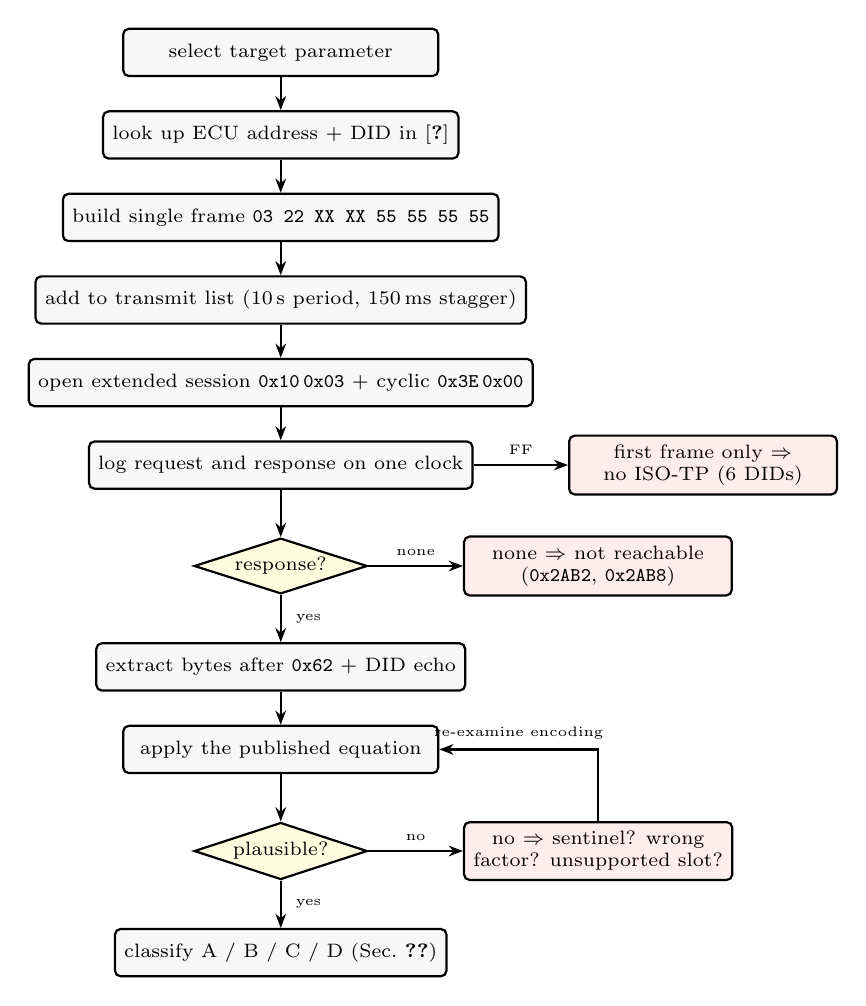
\begin{tikzpicture}[
  font=\scriptsize, node distance=4.2mm,
  st/.style={draw,thick,rounded corners=2pt,minimum height=6mm,minimum width=40mm,align=center,fill=gray!6},
  dc/.style={draw,thick,diamond,aspect=2.4,inner sep=0pt,align=center,fill=yellow!12,minimum width=22mm},
  bad/.style={st,fill=red!7,minimum width=34mm},
  ar/.style={-{Stealth[length=1.8mm]},thick}]

\node[st] (a) {select target parameter};
\node[st,below=of a] (b) {look up ECU address + DID in~\cite{vwmebpidlist}};
\node[st,below=of b] (c) {build single frame \texttt{03 22 XX XX 55 55 55 55}};
\node[st,below=of c] (d) {add to transmit list (10\,s period, 150\,ms stagger)};
\node[st,below=of d] (e) {open extended session \hex{10}\,\hex{03} + cyclic \hex{3E}\,\hex{00}};
\node[st,below=of e] (f) {log request and response on one clock};
\node[dc,below=6mm of f] (g) {response?};
\node[st,below=6mm of g] (h) {extract bytes after \hex{62} + DID echo};
\node[st,below=of h] (i) {apply the published equation};
\node[dc,below=6mm of i] (j) {plausible?};
\node[st,below=6mm of j] (k) {classify A / B / C / D (Sec.~\ref{sec:validation})};

\node[bad,right=12mm of g] (g1) {none $\Rightarrow$ not reachable\\(\hex{2AB2}, \hex{2AB8})};
\node[bad,right=12mm of f] (g2) {first frame only $\Rightarrow$\\no ISO-TP (6 DIDs)};
\node[bad,right=12mm of j] (j1) {no $\Rightarrow$ sentinel? wrong\\factor? unsupported slot?};

\foreach \x/\y in {a/b,b/c,c/d,d/e,e/f,f/g,h/i,i/j} \draw[ar] (\x) -- (\y);
\draw[ar] (g) -- node[right=0.6mm,font=\tiny]{yes} (h);
\draw[ar] (j) -- node[right=0.6mm,font=\tiny]{yes} (k);
\draw[ar] (g) -- node[above,font=\tiny]{none} (g1);
\draw[ar] (f.east) -- node[above,font=\tiny]{FF} (g2);
\draw[ar] (j) -- node[above,font=\tiny]{no} (j1);
\draw[ar] (j1.north) |- node[above,font=\tiny,pos=0.75]{re-examine encoding} (i.east);
\end{tikzpicture}
\caption[UDS acquisition and decoding workflow]{The acquisition and decoding workflow, including the three failure branches the campaign exercised. Every branch produced results that are reported in Chapter~4: two identifiers were never answered, six were truncated for want of a transport layer, and three returned a physically impossible value that turned out to be a reserved not-available code.}
\label{fig:uds_flow}
\end{figure}

The transmit list is provided to the device as a JSON configuration on the SD card. Listing~\ref{lst:canedge_cfg} shows the two settings that had to be changed from the factory default to make active diagnostics possible, and Listing~\ref{lst:canedge_tx} shows the structure of a single transmit entry.

\begin{lstlisting}[float=htbp,caption={CANedge2 PHY configuration changes required for UDS transmission. The factory default is restricted (listen-only) PHY mode with auto bit-rate detection, which never lets the controller transmit.},label={lst:canedge_cfg}]
"can_1": {
  "phy": {
    "mode": 0,                  // Normal; default 1 = Restricted (cannot transmit)
    "retransmission": 1,
    "fd_spec": 0,
    "bit_rate_cfg_mode": 1,     // manual; default 0 = auto-detect
    "bit_rate_std": 500000,     // arbitration rate, matches the ID. Buzz
    "bit_rate_fd": 2000000      // set only so the controller initialises
  },
  "filter": {                   // pass-all: nothing is discarded
    "remote_frames": 0,
    "id": [
      { "name": "AllStandardID", "state": 1,
        "id_format": 0, "f1": "0", "f2": "7FF" },
      { "name": "AllExtendedID", "state": 1,
        "id_format": 1, "f1": "0", "f2": "1FFFFFFF" }
    ]
  }
}
\end{lstlisting}

The two configuration changes in Listing~\ref{lst:canedge_cfg} are what turn the logger from an observer into a participant on the bus. In its factory-default restricted, listen-only PHY mode the controller acknowledges nothing and never drives the bus, so switching \texttt{mode} to Normal is a precondition for the transmit list to have any effect at all. Setting the bit rate to manual rather than auto-detect makes the controller go bus-active immediately at the known 500~kbit/s of the ID.~Buzz diagnostic bus, instead of waiting to infer the rate from existing traffic -- important here because the logger may be the only active diagnostic node and there may be little traffic to detect. The CAN-FD data rate is defined only so that the controller initialises cleanly; CAN-FD itself is unused, since the diagnostic bus is Classical CAN.

The acceptance filters deserve a brief note because they determine what reaches the file. Both channels are configured to pass everything -- one range covering all 11-bit identifiers (\hex{000}--\hex{7FF}) and one covering all 29-bit identifiers (\hex{00000000}--\hex{1FFFFFFF}) -- so no frame is discarded in the logger. This is a deliberate choice: filtering at the device would have been a small bandwidth saving, but it would also have silently removed the unsolicited broadcast traffic whose absence of battery content is itself a result (Section~\ref{ssec:broadcast}). Any selection of what is relevant is therefore made offline, on a complete recording, where it can be revisited.

\begin{lstlisting}[float=htbp,caption={[Transmit-list entries]The first four entries of the 62-entry transmit list, from the deployed \texttt{config-01.08.json}. The fields common to every entry are factored into the comment for brevity.},label={lst:canedge_tx}]
"transmit": [
  // every entry additionally carries "state":1, "id_format":1,
  // "frame_format":0, "brs":0, "log":1, "period":10000
  { "name": "BMS_DiagSessExt", "delay": 0,
    "id": "17FC007B", "data": "0210035555555555" },  // SID 10 03: extended session
  { "name": "BMS_TP",          "delay": 150,
    "id": "17FC007B", "data": "023e005555555555" },  // SID 3E 00: TesterPresent
  { "name": "SOC_BMS_028C",    "delay": 300,
    "id": "17FC007B", "data": "0322028c55555555" },  // SF 03, SID 22, DID 028C
  { "name": "HV_Volt_1E3B",    "delay": 450,
    "id": "17FC007B", "data": "03221e3b55555555" }   // SF 03, SID 22, DID 1E3B
  // ... 58 further 0x22 reads, delay 600 ... 9150 ms
]
\end{lstlisting}

A single transmit entry, as shown in Listing~\ref{lst:canedge_tx}, encodes everything the logger needs to issue one diagnostic read autonomously (the fields identical across all 62 entries are omitted there for brevity): the target request identifier and its format, the exact eight-byte frame to send, and the timing with which to repeat it. The identifier is given as a hexadecimal string holding the 29-bit extended address of the target ECU, and the eight-byte \texttt{data} field carries the single-frame diagnostic payload -- the PCI byte, the ReadDataByIdentifier service, the two-byte Data Identifier and the \hex{55} padding that fills the frame to its full length. The \texttt{delay} field staggers the entry within the 10\,s cycle, and \texttt{log} instructs the device to record the transmitted frame alongside the received ones, which is what allows a request and its response to be paired within a single file. Together the entries form a self-contained schedule that the CANedge2 replays cyclically for the whole recording, with each entry's period and stagger chosen as described above.

Because 62 usable entries cannot cover every cell voltage and every temperature point at once, several configurations were prepared: a \texttt{smoketest} (five reads plus TesterPresent) to verify bus, bit rate and extended-ID addressing before committing to a long recording; a \texttt{drive} configuration weighted towards system-wide signals; and complementary \texttt{cells-front}/\texttt{cells-rear} configurations intended to walk the cell array across successive sessions. All share an identical five-signal core (SOC \hex{028C}, HV voltage \hex{1E3B}, HV current \hex{1E3D}, main temperature \hex{2A0B}, operating mode \hex{7448}) so that logs from different rotations can be time-aligned. The results reported in Chapter~4 come from a single configuration, \texttt{config-01.08-selected}, which samples 31 of the cell slots together with the temperature, system and non-BMS signals; the cell-array rotation was not carried through to a complete 96-cell data set, and Chapter~4 therefore reports a sample rather than full coverage.

The rotation is a direct response to the arithmetic of the problem: the number of quantities worth reading -- 96 cell voltages, 18 temperature points and a set of system-level and non-BMS signals -- far exceeds the 62 usable entries of a single transmit list, so full coverage would require partitioning the reads across several configurations recorded in separate sessions. Beginning with a minimal \texttt{smoketest} confirms the fundamentals of the setup -- that the bus is reachable, the bit rate is correct and the extended-ID addressing of the BMS works -- before committing to the longer sweeps, so that a misconfiguration is caught cheaply rather than after a full recording. Embedding the same five-signal core in every configuration is what makes the separately recorded sessions comparable: because SOC, high-voltage voltage and current, main temperature and operating mode are captured in all of them, the logs share a common set of reference signals along which they can be time-aligned, and the per-configuration cell and temperature data can be related to a consistent battery state.

A known limitation of this hardware-based approach is that the CANedge2 transmit list sends \emph{single} CAN frames only; it has no ISO-TP segmentation. DIDs whose response exceeds 7~payload bytes (for example VIN \hex{F802} or the battery serial number) would return only their first frame and are therefore deliberately excluded from the sweep. This is the direct practical consequence of the OBD-II bus being Classical CAN rather than CAN-FD. A Classical CAN frame carries at most eight payload bytes, so any diagnostic response longer than that must be split across multiple frames and reassembled by the transport layer defined in ISO~15765-2~\cite{iso15765}, which coordinates the multi-frame exchange through flow-control frames between tester and ECU. Because the transmit list can only emit isolated single frames and cannot participate in that flow-control handshake, a multi-frame response is truncated to its first frame. Rather than attempt to work around this in hardware that does not support it, the sweep is confined to identifiers whose answers fit within a single frame, which covers the battery quantities that are the focus of this thesis and leaves only a small number of long, multi-frame identifiers out of reach.

% ============================================================

% ============================================================
\chapter{Results}
% ============================================================
This chapter presents the measurement results of the active UDS reverse engineering. Where the preceding chapters established \emph{how} the battery data can be reached actively and \emph{which} Data Identifiers were selected, the purpose of this chapter is to report \emph{what} the vehicle actually returned and to demonstrate that the decoded quantities correspond to the real physical state of the pack. Section~4.1 gives an overview of the UDS logging campaign and the sessions on which the analysis rests; Section~4.2 reports the response coverage, the battery parameters decoded from the BMS, the anomalies encountered, and the validation of the decoded values against the physical state of the vehicle. Throughout, the emphasis is not merely on presenting numbers but on establishing that each number is trustworthy: because the manufacturer Data Identifiers are undocumented, a decoded value only becomes evidence once its byte layout, scaling, and plausibility have all been confirmed.

\section{UDS Logging Campaign}
The active UDS retrieval produced a set of MF4 logs in which the CANedge2 both transmitted the 59 requests and recorded the BMS responses on the same OBD-II diagnostic bus. This dual role of the logger---transmitter and recorder in one device---is what distinguishes the active campaign from a purely passive capture: every response frame in the log can be attributed unambiguously to the request that immediately preceded it, because the transmit schedule is deterministic and each Data Identifier is echoed back in the positive response. The requests were emitted on a fixed cadence, each identifier being re-read every ten seconds with the individual transmit-list entries staggered by 150~ms so that the requests do not collide on the bus and each response has time to arrive before the next request is issued. Over a session of several hundred seconds this yields dozens of repeated reads of every identifier, which is what allows the coverage figure to be reported as a stable property of the vehicle rather than an artefact of a single lucky exchange.

The campaign deliberately consisted of several recordings taken under the same vehicle condition---the ID.~Buzz drive-ready but stationary, at 72--73\,\% state of charge---rather than a single long log. Repeating the capture serves as a control: if the response coverage and the decoded values are reproducible across independent sessions of different lengths, then the extraction procedure itself is robust and the results are not sensitive to transient bus conditions, timing jitter, or a particular moment in the vehicle's internal state machine. Table~\ref{tab:uds_logs} summarises the sessions used for the analysis. The frame counts listed include the transmitted requests, the logged responses and the unsolicited broadcast traffic that is present on the diagnostic bus, all captured on channel~1; the logger records its own transmitted frames alongside the received ones and tags them with a direction flag, so a request and its answer can be paired within one file. Channel~2 was not connected to any bus and contributes no frames. The longest usable session (\texttt{00000039}, 533~s, 21\,438~frames) is taken as the representative log for the decoded values in Section~4.2 because its longer observation window contains the largest number of repeated reads per identifier and therefore offers the most confidence that a value is steady rather than momentary; the shorter sessions (\texttt{00000040} and \texttt{00000041}) confirm that the response coverage (52/60 positive) is stable across recordings and is not an accident of duration.

\begin{table}[H]
\caption{UDS logging sessions recorded on the VW ID.~Buzz (device \texttt{2A73E1CC}). Frame counts include the transmitted requests, the logged responses and the broadcast traffic present on the diagnostic bus.}
\label{tab:uds_logs}
\centering
\begin{tabular}{lrrl}
\toprule
\textbf{Log} & \textbf{Duration\,[s]} & \textbf{Frames} & \textbf{Positive responses} \\
\midrule
\texttt{00000039} & 533.5 & 21\,438 & 52 / 60 \\
\texttt{00000040} & 333.3 & 12\,630 & 52 / 60 \\
\texttt{00000041} & 233.1 &  8\,526 & 52 / 60 \\
\bottomrule
\end{tabular}
\end{table}

\subsection{Broadcast Traffic Observed at the Diagnostic Connector}
\label{ssec:broadcast}
Research question~1 asks which bus is exposed at the OBD-II connector and why the raw BMS frames are not observable on it. The logs answer the first half directly and constrain the second. The diagnostic bus is \emph{not} silent: alongside the diagnostic exchange, log \texttt{00000039} contains 14\,921 unsolicited broadcast frames distributed over six standard 11-bit identifiers -- \hex{065} (2652 frames), \hex{066} (2561), \hex{067} (2341), \hex{068} (2341), \hex{06B} (2340) and \hex{06F} (2686). The gateway therefore does forward \emph{some} broadcast traffic outward.

None of it, however, could be attributed to the battery. These six identifiers were examined byte-wise during the exploratory phase of this work; their payloads change on time scales inconsistent with the quantities of interest, and no byte or byte pair within them tracks any of the battery parameters that the UDS reads recover in the same recording -- neither the state of charge, nor the pack voltage, nor any cell voltage or temperature. The claim that this thesis makes is therefore the narrow one that the evidence supports: \textbf{the broadcast traffic reaching the OBD-II connector does not carry the BMS measurement frames}, and a passive byte-level reverse engineering of the battery signals at this connector has nothing to work with. Whether the gateway suppresses those frames deliberately, or whether they are simply absent from the bus segment the connector taps, cannot be distinguished from outside the vehicle. This is a negative result, but it is the result on which the entire active methodology rests, and it is reported here rather than assumed.

\section{Active Battery Data Retrieval via UDS}
Following the procedure described in Section~\ref{sec:uds_procedure}, the CANedge2 transmit list was deployed with the 60 selected Data Identifiers of Table~\ref{tab:selected_signals} and the resulting MF4 logs were decoded with \texttt{asammdf}~\cite{asammdf}. The decoding pipeline parses the MDF~4.11 container, isolates the diagnostic response frames by their extended reply identifier, reassembles the payload of each single-frame response, and applies the per-DID scaling from the master PID list to obtain a physical quantity. This section reports the values that were actually extracted from the vehicle, beginning with how completely the vehicle answered the request set, then the decoded parameters themselves, the anomalous identifiers that must be excluded, and finally the validation of the surviving values against the physically observable state of the car.

\subsection{Response Coverage}
\label{ssec:coverage}
Across the logging sessions, of the 60~selected identifiers, \textbf{52~returned a positive single-frame response} -- of which, as Section~\ref{ssec:anomalies} shows, only 49 carry a usable value. Coverage is reported first because it bounds everything that follows: an identifier that never answered, or that answered only partially, cannot contribute a validated value regardless of how attractive the parameter it names might be. The reassuring finding is that the same 52 identifiers succeeded in every session (Table~\ref{tab:uds_logs}), so the eight that did not succeed are a systematic property of the interface rather than random loss. The remaining identifiers fall into two groups that are entirely explained by the hardware:

\begin{itemize}
  \item \textbf{Six identifiers} (\hex{2AF7}~12\,V voltage, \hex{0800}~A/C compressor, \hex{F802}~VIN, \hex{0500}~battery serial, \hex{1E32}~cumulative charge/dis\-charge, \hex{1E3D}~pack current) returned only their First Frame. As predicted in Section~\ref{sec:uds_procedure}, the CANedge2 transmit list has no ISO-TP support, so any response longer than 7~payload bytes is truncated.
  \item \textbf{Two identifiers} (\hex{2AB2}, \hex{2AB8}~energy content) returned neither a positive nor a negative response.
\end{itemize}

The first group is a direct and predictable consequence of the transport layer rather than of the vehicle. Under ISO~15765-2~\cite{iso15765}, a diagnostic message whose payload fits in seven bytes is sent as a single frame, but any longer message is segmented into a First Frame followed by Consecutive Frames, and the receiver of the First Frame is obliged to return a Flow Control frame before the sender continues. The CANedge2 transmit list can emit only fixed single CAN frames on a fixed schedule; it cannot generate the Flow Control frame that the BMS waits for, so the ECU sends its First Frame---carrying the length header and the first six payload bytes---and then stalls, and only that First Frame is logged~\cite{csselectronics_canedge2}. It is no coincidence that exactly these six identifiers are affected: they name quantities that are intrinsically longer than seven bytes. The VIN (\hex{F802}) is a 17-character string, the battery serial (\hex{0500}) is a comparable identifier string, the cumulative charge/discharge counters (\hex{1E32}) and the energy fields are wide integers that accumulate over the pack's life, and the instantaneous pack current (\hex{1E3D}) is returned in a multi-value record. None of these could ever fit in a single frame, so their truncation is a limitation of the logging tool, not evidence that the data is unavailable in the vehicle; a tester with a full ISO-TP~\cite{iso15765} stack would retrieve them completely.

The second group is qualitatively different and more informative. The two energy-content identifiers (\hex{2AB2}, \hex{2AB8}) produced neither a positive response nor a negative response code. A negative response such as NRC~\hex{31} (\emph{requestOutOfRange}) would have indicated that the addressed ECU recognised the request but rejected the identifier; complete silence says less. Two observations narrow the possibilities. First, the addressing is demonstrably correct: all three identifiers directed at the gateway \hex{710} were transmitted 53~times each in log~\texttt{00000039}, and one of them (\hex{2AF7}, 12\,V battery voltage) answered every time on \hex{77A}. The control unit is present, reachable and listening. Second---and this is a limitation of the experiment rather than a property of the vehicle---no extended diagnostic session was opened on \hex{710}, and no TesterPresent was sent to it; only the BMS received session control (Section~\ref{sec:uds_procedure}). A session-state cause therefore cannot be excluded, and the honest conclusion is that these two identifiers were \emph{not reachable under the conditions tested}. Distinguishing an unimplemented identifier from one that requires a non-default session would require repeating the sweep with session control extended to \hex{710}; this was not done and is recommended in Section~\ref{sec:outlook}. Note also that the source list~\cite{vwmebpidlist} marks both identifiers ``equation missing'', so no decoding could have been attempted even had they answered. Taken together, the coverage result is precisely what the method predicts: everything that is a short, single-frame scalar on the addressed BMS was retrieved, everything intrinsically multi-frame was truncated by the absence of ISO-TP, and a small residue is simply not exposed at this diagnostic endpoint.

\subsection{Extracted Battery Parameters}
Table~\ref{tab:uds_results} lists the physical values decoded from a representative session (log \texttt{00000039}, 533.5~s, 21\,438 frames, 72.8--73.2\,\% SOC), obtained by applying the equations of the community list~\cite{vwmebpidlist} to the raw bytes of each positive response. Each value is reported as the range observed over the 53--54 repeated reads within the session.

The outcome of the sweep is summarised in Figure~\ref{fig:did_coverage}, which breaks the 60~identifiers down by the control unit addressed and by what came back. Two features are worth noting before the values themselves. First, the reads are not all directed at the battery: 53~go to the BMS, the remaining seven to three other control units, and every read that failed outright belongs to the one ECU that was queried without session control. Second, the headline figure of 52~positive responses overstates the usable yield, because three of those responses carry a reserved not-available code rather than a measurement (Section~\ref{ssec:anomalies}); the number of identifiers that actually produced a value is 49.

The small spans in the table are of two kinds, and the distinction matters when judging stability. The state of charge steps once, monotonically, from 73.2\,\% to 72.8\,\% -- a single quantisation step of the raw byte from 183 to 182, consistent with a slow net discharge that the 0.4\,\%\,/\,LSB resolution can barely resolve over 533~s. The pack voltage, by contrast, dithers non-monotonically by $\pm$1~LSB (0.25~V) about roughly 373.4~V, which is measurement noise rather than a trend. Figure~\ref{fig:session_stability} shows both, together with the thermal channels and the 12\,V rail.

The cell-voltage identifiers require care on two counts. The transmit list does not read every cell: to stay within the 64-entry budget it samples 31~of the available slots, roughly every third one, spanning indices 1 to 104. What the table reports is therefore a \emph{sample} of the cell array, not a contiguous block, and any statement about the pack as a whole must be qualified accordingly. Across the 28~sampled slots that returned a plausible value, the readings span 3.888--3.890~V with a mean of 3.8891~V and an inter-cell spread of only 2.8~mV (Figure~\ref{fig:cell_map}). Because each individual cell also jitters by $\pm$2--3~mV between successive reads, this spread sits at or below the temporal noise floor of the measurement: the correct conclusion is not that the cells are identical, but that \textbf{any imbalance present is smaller than this method can resolve}.

The thermal identifiers tell a coherent story of their own. The main battery temperature (\hex{2A0B}, 16.0~\textdegree C) sits inside the range of the seven sampled distributed temperature points (\hex{1EAE} and following plus \hex{7426}, 16.00--16.38~\textdegree C), and the extreme-temperature identifiers \hex{1E0E}/\hex{1E0F} bracket them at 16.375~\textdegree C and 15.875~\textdegree C -- a consistency check between two independently decoded groups. All lie a little below the outdoor reading (\hex{2609}, 16.5--18.0~\textdegree C), as expected for a pack with substantial thermal mass, and the PTC heater draws 0.0~A because no conditioning was active. Note that \hex{1E0E}/\hex{1E0F} use a scale factor of $1/64$ rather than the $1/8$ with an offset of $-40$ used by the temperature points; applying the latter would yield roughly 91~\textdegree C, and it is the disagreement with the independently read points that identifies the correct factor.

\begin{figure}[H]
\centering
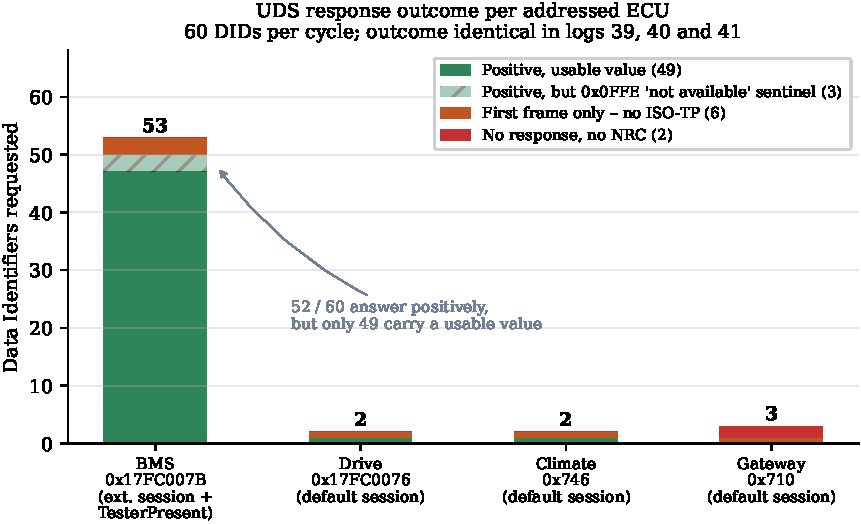
\includegraphics[width=0.92\textwidth]{new_did_coverage.pdf}
\caption[UDS response outcome per addressed ECU]{Outcome of the 60~identifier reads per addressed control unit, identical across logs \texttt{00000039}, \texttt{00000040} and \texttt{00000041}. Only the BMS was placed in an extended diagnostic session; the two identifiers that produced no response at all belong to the gateway, which was queried in the default session.}
\label{fig:did_coverage}
\end{figure}

\begin{figure}[H]
\centering
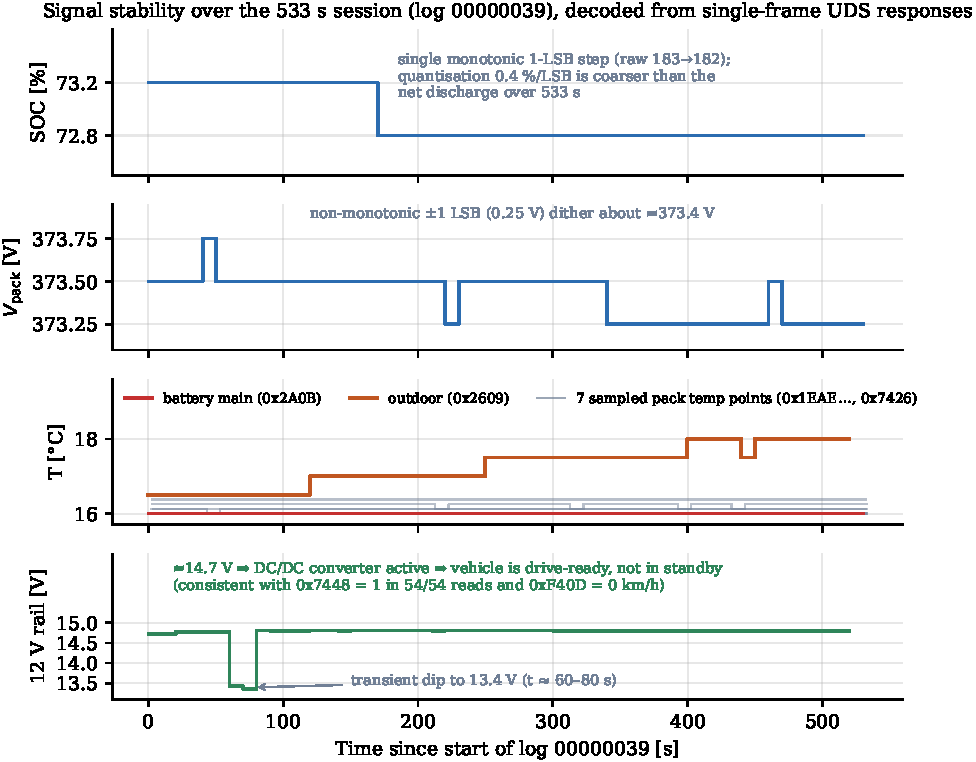
\includegraphics[width=0.95\textwidth]{new_session_stability.pdf}
\caption[Signal stability over the 533\,s session]{Decoded signals over log \texttt{00000039}. The state of charge steps once by one quantisation level; the pack voltage dithers by $\pm$1~LSB about 373.4~V. The 12\,V rail at $\approx$14.7~V indicates an active DC/DC converter, which together with \hex{7448}~$=$~1 and \hex{F40D}~$=$~0\,km/h establishes that the vehicle was drive-ready and stationary rather than in standby.}
\label{fig:session_stability}
\end{figure}

\begin{table}[H]
\caption[Decoded battery parameters]{Parameters decoded from log \texttt{00000039}. Scalings are those published in the community identifier list~\cite{vwmebpidlist} unless marked~$\dagger$, which denotes an encoding recovered in this work. Values are the range over the 53--54 repeated reads in the session.}
\label{tab:uds_results}
\centering\small
\begin{tabular}{@{}llll@{}}
\toprule
\textbf{Parameter} & \textbf{DID} & \textbf{Scaling} & \textbf{Measured} \\
\midrule
\multicolumn{4}{@{}l}{\itshape Pack level} \\
State of charge (BMS)              & \hex{028C} & raw$/2.5$ [\%]                     & 72.8--73.2\,\% \\
Pack voltage                       & \hex{1E3B} & raw$_{16}/4$ [V]                   & 373.25--373.75\,V \\
Dynamic charge limit               & \hex{1E1B} & raw$_{16}/5$ [A]                   & 352.4--355.2\,A \\
Dynamic discharge limit            & \hex{1E1C} & raw$_{16}/5$ [A]                   & 800.0\,A (constant) \\
\midrule
\multicolumn{4}{@{}l}{\itshape Cell level} \\
Cell voltage, 28 sampled slots     & \hex{1E40}$+n-1$ & raw$_{16}/1000+1$ [V]        & 3.888--3.890\,V \\
Highest cell (voltage; index)      & \hex{1E33} & raw$_{16}/4096$ [V]~$\dagger$; \texttt{B[3]} & 3.889--3.894\,V; cells 3--82 \\
Lowest cell (voltage; index)       & \hex{1E34} & raw$_{16}/4096$ [V]~$\dagger$; \texttt{B[3]} & 3.881--3.885\,V; \textbf{cell 96} \\
Slots 97, 100, 104                 & \hex{1EA0},\hex{1EA3},\hex{1EA7} & raw $=$ \hex{0FFE}~$\dagger$ & not available \\
\midrule
\multicolumn{4}{@{}l}{\itshape Thermal} \\
Battery temperature (main)         & \hex{2A0B} & raw$/2-40$ [\textdegree C]         & 16.0\,\textdegree C \\
Temp.\ points 1,3,6,9,12,15        & \hex{1EAE}$+$ & raw$_{16}/8-40$ [\textdegree C] & 16.00--16.38\,\textdegree C \\
Temp.\ point 18                    & \hex{7426} & raw$_{16}/8-40$ [\textdegree C]    & 16.00--16.12\,\textdegree C \\
Highest temp.\ (value; point)      & \hex{1E0E} & raw$_{16}/64$; \texttt{B[3]}       & 16.375\,\textdegree C; pt.\ 5--6 \\
Lowest temp.\ (value; point)       & \hex{1E0F} & raw$_{16}/64$; \texttt{B[3]}       & 15.875\,\textdegree C; pt.\ 3--7 \\
Outdoor temperature                & \hex{2609} & raw$/2-50$ [\textdegree C]         & 16.5--18.0\,\textdegree C \\
PTC heater current                 & \hex{1620} & raw$/4$ [A]                        & 0.0\,A \\
\midrule
\multicolumn{4}{@{}l}{\itshape Vehicle state} \\
Car operation mode                 & \hex{7448} & enum \{0,1,4,6\}                   & \textbf{1 (driving), 54/54} \\
Speed                              & \hex{F40D} & raw [km/h]                         & 0 (constant) \\
\bottomrule
\end{tabular}
\end{table}

A representative single-frame exchange for the pack voltage (DID \hex{1E3B}) is:

\begin{lstlisting}[float=htbp,caption={Raw UDS exchange for the pack voltage DID, as logged by the CANedge2.},label={lst:uds_voltage}]
>>> 03 22 1E 3B 55 55 55 55     # SF, len=3, SID=22 (Read), DID=1E3B, 0x55 padding
<<< 05 62 1E 3B 05 D5 aa aa     # SF, len=5, SID=62 (pos), payload 0x05D5
                                # 0x05D5 = 1493 -> 1493/4 = 373.25 V
\end{lstlisting}

Listing~\ref{lst:uds_voltage} makes the decoding chain explicit and shows why a single successful exchange already contains everything needed to trust the value. The request is a single frame whose first byte \hex{03} is the ISO~15765-2 protocol control information declaring three payload bytes, followed by the UDS \texttt{ReadDataByIdentifier} service \udssid{22} and the two-byte identifier \hex{1E3B}, with the remaining bytes filled by the VW padding value \hex{55}. The response echoes the identifier back after a service byte of \udssid{62}---the request service \udssid{22} plus the \hex{40} offset that ISO~14229~\cite{iso14229} prescribes for a positive response---which is what allows every response in the log to be matched to its request without ambiguity. The two payload bytes \hex{05}\hex{D5} form the raw 16-bit value 1493, and dividing by the reconstructed scale factor of four yields 373.25~V, a figure that lands squarely inside the pack-voltage range of the table. The echoed identifier and the deterministic service offset are precisely the features that make the active method self-labelling: unlike a passively sniffed broadcast frame, whose meaning must be guessed from context, a UDS response carries its own identifier and thereby its own provenance.

\subsection{The Cell-Extreme Identifiers: an Encoding the Source List Omits}
\label{ssec:cellextremes}
The community list~\cite{vwmebpidlist} describes \hex{1E33} and \hex{1E34} only as ``the cell \# with highest / lowest voltage'', documenting the trailing byte \texttt{ZZ} of the four-byte response and labelling the identifiers, evidently in error, with the unit \textdegree C. The response is longer than that description accounts for. A representative exchange is

\begin{center}
\ttfamily 07 62 1E 33 3E 4A 00 52 \qquad and \qquad 07 62 1E 34 3E 25 00 60
\end{center}

\noindent so four data bytes \texttt{WW XX YY ZZ} follow the echoed identifier, of which the list explains one. Reading \texttt{ZZ} gives cell~\hex{52}~$=$~82 and cell~\hex{60}~$=$~96 respectively. The leading pair \texttt{WW XX} was recovered here: interpreted as a 16-bit big-endian integer and divided by 4096, \hex{3E4A} yields 3.8931~V and \hex{3E25} yields 3.8840~V. Both land squarely in the cell-voltage band, and the scale factor 4096 differs from the 1000 used by the individual cell identifiers, so it could not have been guessed from them.

The interpretation is confirmed by a relation that neither decoding knows about. The 28~individually sampled cells of Section~\ref{ssec:coverage} span 3.888--3.890~V; the extremes reported by \hex{1E33}/\hex{1E34} over the same session span 3.881--3.894~V. The reported extremes \emph{bracket} the independent sample, which is exactly what a maximum and a minimum over the full cell array must do with respect to a subset of it, and would not occur for an arbitrary scale factor. Figure~\ref{fig:cell_map} shows this graphically.

A caution belongs here. An earlier decoding of these identifiers in this work read the \emph{first} data byte rather than the last and reported ``cell~62'' for both -- \hex{3E}~$=$~62 being the high byte of the voltage field, not an index at all. The error was self-revealing: the highest-voltage and the lowest-voltage cell cannot be the same cell unless every cell is exactly equal, and the per-cell data show they are not. The episode illustrates why a decoded value is not evidence until it has been checked against something the decoder could not have produced.

Across all three sessions the identity of the extreme cells is itself informative. The highest-voltage cell wanders -- cells 3, 5, 10, 11, 13, 30, 44, 58, 60, 70, 74 and 82 all appear -- which is what one expects when the spread between cells is comparable to the measurement resolution and the position of the maximum is decided by noise. The lowest-voltage cell does not wander: \hex{1E34} reports \textbf{cell~96 in every one of the 112~reads across logs \texttt{00000039}, \texttt{00000040} and \texttt{00000041}} (Figure~\ref{fig:cell_extremes}). Cell~96 is consistently the weakest cell in this pack. The margin is small -- of the order of 10~mV below the maximum -- and at 72\,\% SOC with the vehicle stationary it carries no immediate implication for the health of the pack, but it is a stable, reproducible observation of exactly the kind that a longitudinal fleet measurement would be built on.

\subsection{Anomalies: the \hex{0FFE} Not-Available Code}
\label{ssec:anomalies}
Three of the sampled cell-voltage identifiers (\hex{1EA0}~slot~97, \hex{1EA3}~slot~100, \hex{1EA7}~slot~104) return a constant raw value of \hex{0FFE} in every one of their 53~reads, which under the cell-voltage equation would decode to 5.094~V -- far outside the physically possible range of a lithium-ion cell, whose open-circuit terminal voltage stays well below 4.3~V even when fully charged.

The reading is diagnostically useful precisely because it is impossible, and the raw value identifies the mechanism. \hex{0FFE} is one below \hex{0FFF}, the largest value a 12-bit field can hold. Reserving the top codes of a fixed-width field to signal ``not available'' or ``error'' rather than a measurement is a standard convention in automotive signal encoding, and the observation is consistent with it in three respects: the value is bit-exact and never varies, it appears only at slot indices above 96, and it appears on identifiers that are otherwise addressed and answered normally. The identifiers are therefore not mis-scaled and not broken -- they are \emph{working correctly and reporting that there is nothing to report}, because the pack does not populate those slots. Note that this contradicts the natural first hypothesis, which is that the raw value simply does not follow the same scaling; it does follow it, and the point is that the code lies outside the range the scaling is defined over.

The criterion applied here is stated explicitly so that it can be checked: \textbf{a value is classified as a sentinel rather than a measurement when it is bit-exact across every read of every session, lies at or adjacent to the maximum of its field width, and decodes to a physically impossible quantity}. All three conditions hold for \hex{0FFE} on these identifiers, and no other identifier in the sweep meets them. Such identifiers are excluded from the results rather than rescaled; forcing a scaling onto them would be the error the criterion exists to prevent.

\subsection{The Number of Cell-Voltage Channels}
\label{ssec:cellcount}
The manufacturer does not publish how many individual cell voltages the ID.~Buzz battery-management system measures, and the figure matters: it is needed to relate the per-cell readings to the pack voltage, and it bounds the address space worth sweeping. Three independent lines of evidence in the data converge on the same answer.

\begin{enumerate}
  \item \textbf{From above.} Slots 97, 100 and 104 return the \hex{0FFE} not-available code in 100\,\% of reads (Section~\ref{ssec:anomalies}). Whatever the pack contains, it does not populate slot~97 or beyond.
  \item \textbf{From below.} The lowest-voltage identifier \hex{1E34} names cell~96 in all 112 reads across three sessions (Section~\ref{ssec:cellextremes}). Cell~96 therefore exists and is measured. Together with the previous point this brackets the count at exactly 96.
  \item \textbf{From the pack voltage.} The mean of the 28~sampled cells is 3.8891~V and the measured pack voltage is 373.25--373.75~V, giving a ratio of 95.95--96.08. Figure~\ref{fig:series_count} plots the predicted pack voltage $N\times\overline{V}_\mathrm{cell}$ against the assumed series count: $N=95$ predicts 369.5~V and $N=97$ predicts 377.2~V, both far outside the measured band, while $N=96$ predicts 373.35~V, inside it.
\end{enumerate}

\noindent The three arguments are independent -- one rests on a sentinel code, one on an index reported by the BMS itself, and one on the ratio of two separately decoded analogue quantities -- and they agree. The battery-management system of this vehicle is concluded to expose \textbf{96 cell-voltage channels}, consistent with a series string of 96 parallel cell groups. This also resolves what the identifier block size does \emph{not} mean: the cell identifiers occupy a contiguous address range extending well beyond \hex{1EA0}, and the size of that range reflects the largest pack variant the firmware supports, not the hardware of this vehicle.

\begin{figure}[H]
\centering
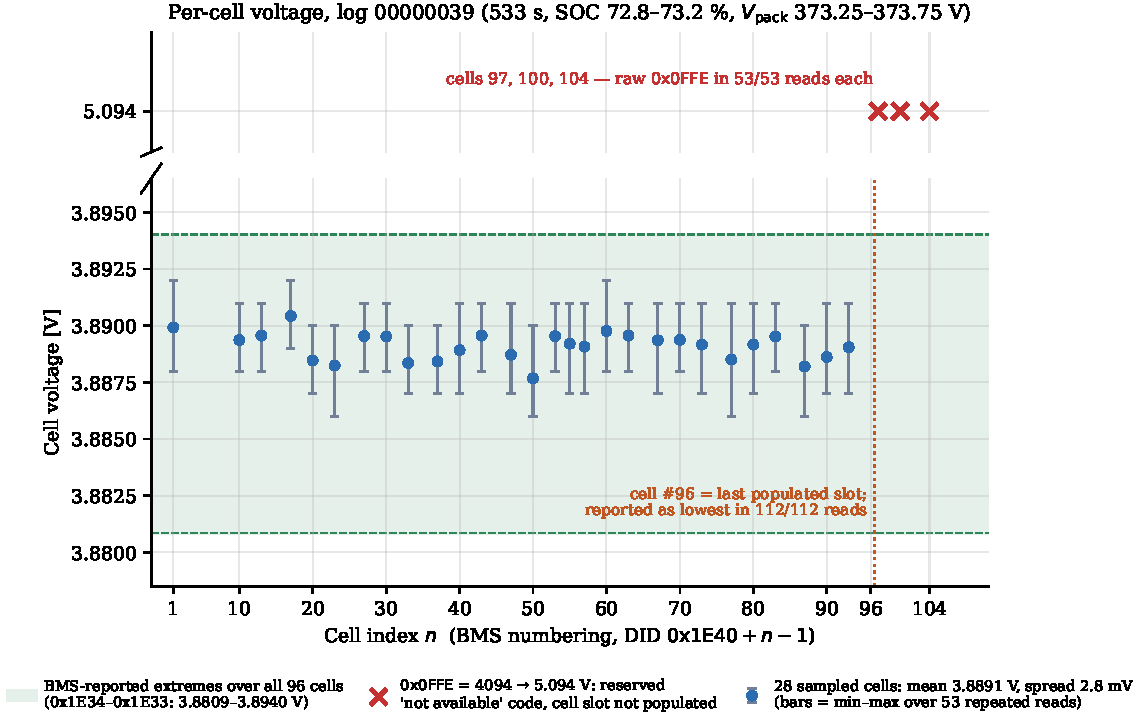
\includegraphics[width=0.98\textwidth]{new_cell_voltage_map.pdf}
\caption[Per-cell voltage and the boundary of the populated address space]{Per-cell voltage decoded from log \texttt{00000039}. The 28~sampled slots that return a measurement span 2.8~mV, which is comparable to the $\pm$2--3~mV jitter of each individual slot between reads. The band shows the extremes reported independently by \hex{1E34} and \hex{1E33}; that it brackets the sample confirms both decodings. Slots 97, 100 and 104 return the bit-exact \hex{0FFE} not-available code.}
\label{fig:cell_map}
\end{figure}

\begin{figure}[H]
\centering
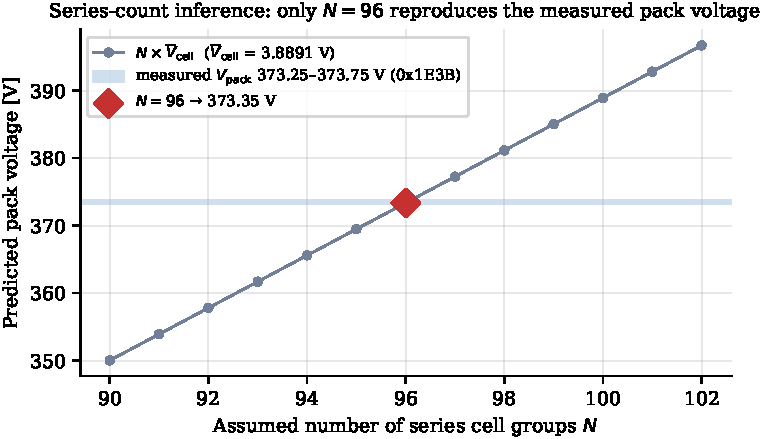
\includegraphics[width=0.78\textwidth]{new_series_count.pdf}
\caption[Series-count inference]{Predicted pack voltage against assumed series count. Only $N=96$ reproduces the measured pack voltage, independently of the two arguments from the identifier space.}
\label{fig:series_count}
\end{figure}

\begin{figure}[H]
\centering
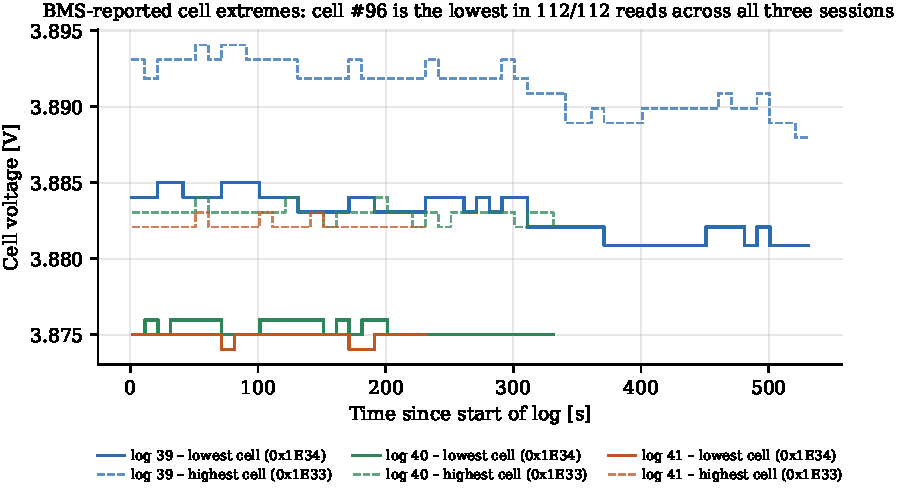
\includegraphics[width=0.95\textwidth]{new_cell_extremes.pdf}
\caption[Reported cell extremes across three sessions]{Cell extremes reported by \hex{1E33}/\hex{1E34}. The highest-voltage cell wanders with the noise; the lowest is cell~96 in all 112~reads across three independent sessions.}
\label{fig:cell_extremes}
\end{figure}

\subsection{Validation Status of the Decoded Signals}
\label{sec:validation}
A decoded value is not evidence until something outside the decoding agrees with it. Any monotonic scaling can turn a raw integer into a number that looks like a voltage, so the question for each signal is what, precisely, is known to be true about it independently of the equation used to produce it. Applying that question honestly to this data set gives four classes, and they are unevenly populated: only two signals reach the strongest class.

\paragraph{Class A -- directly validated.} \hex{7448} (operation mode) and \hex{F40D} (speed). The vehicle was switched on and standing still throughout every recording; this is a fact about the world, established without reference to the CAN bus. \hex{7448} returned the constant value~1 in all 112~reads across the three sessions, which the source list~\cite{vwmebpidlist} maps to \emph{driving} -- that is, drive-ready rather than in motion -- and \hex{F40D} returned 0\,km/h throughout. Both agree with the observed state of the vehicle, and a third decoded signal corroborates them: the 12\,V rail (\hex{2AF7}) sits at $\approx$14.7~V, which requires an active DC/DC converter and is inconsistent with a sleeping vehicle. It must be said plainly that the earlier reading of this signal in the present work was wrong: the recordings were described as having been taken in standby, whereas the vehicle reports itself as drive-ready in every single sample.

\paragraph{Class B -- indirectly validated.} \hex{1E3B} (pack voltage), \hex{1E40}$+$ (cell voltages), \hex{1E33}/\hex{1E34} (cell extremes) and the thermal group \hex{2A0B}, \hex{1EAE}$+$, \hex{7426}, \hex{1E0E}, \hex{1E0F}. These have no external reference, but they are constrained by physical relations that the decodings themselves do not encode. The ratio of the pack voltage to the mean cell voltage is 95.95--96.08, an integer to within 0.1\,\% (Section~\ref{ssec:cellcount}); the BMS-reported cell extremes bracket the independently sampled cells (Section~\ref{ssec:cellextremes}); and the reported temperature extremes bracket the independently sampled temperature points. Two separately decoded quantities satisfying a relation neither was fitted to is strong evidence that both are right. It is not proof: these checks fix the scalings \emph{relative to one another}, and a systematic factor common to a pair would satisfy the relation and still be wrong. No calibrated instrument was applied to the pack, so no absolute anchor exists for any of them.

\paragraph{Class C -- plausible but unconfirmed.} \hex{028C} (SOC), \hex{1E1B}/\hex{1E1C} (power limits), \hex{1620} (PTC current), \hex{2609} (outdoor temperature), \hex{295A} (odometer), \hex{2AF7} (12\,V voltage) and \hex{1E3D} (pack current). Every one of these produces a physically sensible magnitude and none has an independent reference in these recordings.

The state of charge deserves specific comment, because it is the parameter a reader will most expect to see validated and it is the easiest to overstate. The decoded 72.8--73.2\,\% is consistent with the charge level at which the vehicle was left before the session, but \textbf{no photograph of the instrument cluster was taken during these recordings, and no independent state-of-charge readout was captured}. A recollection of the approximate charge level is not a reference measurement, and the value is therefore reported here as plausible and internally stable -- it repeats to within one quantisation step over 533~s and across three sessions -- but \emph{not} as validated. Capturing a synchronised dashboard reading is a trivial addition to a future session and would move this signal to class~A at no cost; that it was not done is a shortcoming of the experimental procedure, not of the decoding.

The 12\,V voltage and the pack current carry a further caveat: both were recovered from a first frame whose continuation was never received. For \hex{2AF7} the two bytes the equation consumes happen to fall inside the first frame, so a value ($\approx$14.7~V, varying over 21~distinct levels) can be computed -- but the remaining 20~bytes of the 26-byte record were never seen, so the assumption that those two bytes occupy the position the list assigns them is untested. For \hex{1E3D} only the leading three of the data bytes arrived, bounding the current to roughly $-5$ to $-2$~A, a magnitude consistent with a stationary vehicle supplying its low-voltage loads but not a measurement.

\paragraph{Class D -- invalid or unexplained.} \hex{1EA0}, \hex{1EA3}, \hex{1EA7} return the \hex{0FFE} not-available code and are excluded (Section~\ref{ssec:anomalies}). \hex{0800} (A/C compressor status on the climate ECU) answers and varies across six distinct payloads, but the source list supplies no equation for it and only its first frame was captured, so it remains uninterpreted. \hex{2AB2} and \hex{2AB8} were never answered under the conditions tested (Section~\ref{ssec:coverage}).

\medskip\noindent
Table~\ref{tab:validation_classes} summarises the classification. The distribution is itself a result, and not a flattering one: of 60~identifiers requested, two are validated against an external fact, roughly a dozen are supported by internal consistency, and the remainder rest on plausibility alone. Stating this is what separates the present work from a list of numbers that merely look correct.

\begin{table}[H]
\caption[Validation status of the decoded signals]{Validation status of every signal recovered in this work. The term \emph{validated} is reserved for class~A.}
\label{tab:validation_classes}
\centering\small
\begin{tabular}{@{}p{2.3cm}p{3.4cm}p{7.4cm}@{}}
\toprule
\textbf{Class} & \textbf{Signals} & \textbf{Basis, and what it does not establish} \\
\midrule
A -- directly validated &
\hex{7448}, \hex{F40D} &
Agree with a fact observable without the bus: the vehicle was on and stationary. The only signals with a wholly independent reference. \\[3pt]
B -- indirectly validated &
\hex{1E3B}, \hex{1E40}$+$, \hex{1E33}, \hex{1E34}, \hex{2A0B}, \hex{1EAE}$+$, \hex{7426}, \hex{1E0E}, \hex{1E0F} &
Mutually consistent under relations the decodings do not encode ($V_\mathrm{pack}/\overline{V}_\mathrm{cell}=95.95$--$96.08$; extremes bracket the samples). Fixes the scalings relative to each other, not absolutely. \\[3pt]
C -- plausible, unconfirmed &
\hex{028C}, \hex{1E1B}, \hex{1E1C}, \hex{1620}, \hex{2609}, \hex{295A}, \hex{2AF7}, \hex{1E3D} &
Physically sensible magnitudes, no independent reference recorded. \hex{2AF7} and \hex{1E3D} additionally rest on an unverified field position within a truncated record. \\[3pt]
D -- invalid / unexplained &
\hex{1EA0}, \hex{1EA3}, \hex{1EA7}, \hex{0800}, \hex{2AB2}, \hex{2AB8} &
Sentinel-coded, or answered without a published equation, or not answered at all. \\
\bottomrule
\end{tabular}
\end{table}

% ============================================================

% ============================================================
\chapter{Discussion}
% ============================================================
\section{Comparison with Related Work}
The passive reverse-engineering literature surveyed in Section~\ref{sec:sota} -- READ~\cite{read}, LibreCAN~\cite{librecan}, CAN-D~\cite{cand} and the machine-learning approach of Huybrechts et al.~\cite{huybrechts2018automatic} -- shares a precondition that the vehicle studied here does not meet. Each assumes the target ECU's broadcast frames can be observed, and each then attacks the genuinely hard problem of segmenting an opaque byte stream into signals. Section~\ref{ssec:broadcast} shows that on the ID.~Buzz the battery frames are simply not present at the diagnostic connector; the six broadcast identifiers that are present carry nothing attributable to the battery. The methods of that literature are therefore not weaker than the one used here -- they are inapplicable at this measurement point, and the comparison is one of preconditions rather than of performance.

The work presented here occupies a different and, it should be said, a less demanding position. Because the acquisition is active, each response arrives labelled: the ECU echoes the requested identifier back, so the segmentation problem that the passive literature exists to solve does not arise. What remains is not signal discovery but \emph{verification}: an identifier list compiled for the VW~ID.3~\cite{vwmebpidlist} proposes an encoding, and the question is whether that proposal holds on a different vehicle. It would misrepresent this thesis to claim otherwise, and the results in Chapter~4 should be read in that light -- the majority of the encodings reported there were adopted from that list and confirmed, not discovered.

Three findings do go beyond the source list, and they are the substantive contribution. The list documents only the trailing index byte of \hex{1E33}/\hex{1E34}; the leading bytes were shown here to carry the cell voltage scaled by $1/4096$, confirmed by the fact that the resulting extremes bracket 28~independently sampled cells (Section~\ref{ssec:cellextremes}). The list documents no sentinel convention; the bit-exact \hex{0FFE} returned by unpopulated slots was identified here as a reserved not-available code at the top of a 12-bit field (Section~\ref{ssec:anomalies}). And the number of cell-voltage channels, which the manufacturer does not publish and the list does not state, was established as 96 by three independent arguments (Section~\ref{ssec:cellcount}). Beyond these, the response-coverage result is itself a transferability measurement: it quantifies how much of an ID.3-derived identifier set survives on an ID.~Buzz, through a production gateway, using a logger with no transport layer.

A word on the community database \texttt{opendbc}~\cite{opendbc} is warranted because it is easily miscited. It is a collection of DBC files describing \emph{broadcast} CAN signals, principally for driver-assistance functions. It contains no UDS Data Identifiers and does not document Volkswagen's \hex{17FC00xx}/\hex{17FE00xx} diagnostic addressing, so it could not have been, and was not, used to cross-check the identifiers of this work. It is cited here only as a representative example of the community signal-database effort of which the ID.3 identifier list is another instance.

\section{Contributions}
The contribution of this thesis is stated here explicitly, and deliberately narrowly, so that it can be assessed against the evidence of Chapter~4 rather than against the ambition of Chapter~1.

\begin{enumerate}
  \item \textbf{A single-device active acquisition method.} Battery data was elicited and recorded through a production gateway using one device. Because the CANedge2 transmit list issues the diagnostic requests itself, no second tester shares the bus, every response is timestamped on the same clock as the request that caused it, and no cross-device time alignment is needed in post-processing. The configuration is portable between vehicles without hardware modification.
  \item \textbf{A transferability measurement.} The response coverage of Section~\ref{ssec:coverage} quantifies how much of an identifier set compiled for the VW~ID.3 survives on a VW~ID.~Buzz when addressed through the OBD-II gateway with a logger that has no transport layer: 52~of 60~identifiers answer, 49~carry a usable value, six are truncated by the absence of ISO-TP, and two are not reachable under the conditions tested. This measurement did not previously exist.
  \item \textbf{Three encodings the source list does not contain.} The $1/4096$ cell-voltage field in the leading bytes of \hex{1E33}/\hex{1E34} (Section~\ref{ssec:cellextremes}); the bit-exact \hex{0FFE} not-available code returned by unpopulated cell slots, together with an explicit criterion for distinguishing a sentinel from a measurement (Section~\ref{ssec:anomalies}); and the determination that the pack exposes 96~cell-voltage channels, established by three independent arguments (Section~\ref{ssec:cellcount}).
  \item \textbf{An explicit validation classification.} Each decoded signal is placed in one of four evidence classes (Section~\ref{sec:validation}), and the term \emph{validated} is reserved for the two signals with a reference independent of the bus. The classification is as much a statement of what is \emph{not} established as of what is.
  \item \textbf{A reproducible tool chain.} The configuration builder, the MF4 reader, the identifier-list decoder and the automated plausibility-check report together turn a raw recording into a classified signal set without manual intervention, and are documented in Section~\ref{sec:toolchain} and Appendix~\ref{app:code}.
\end{enumerate}

\noindent Equally, three things are \emph{not} contributions of this work and are claimed nowhere in it: the byte layouts and scalings of the identifiers adopted from the community list, which were verified here but not discovered; the state of health, which was never requested; and the pack current, whose response is segmented and was therefore never recovered.

\section{Limitations}
Five main limitations of this work should be stated explicitly:

\begin{enumerate}
  \item \textbf{No ISO-TP segmentation.} The decisive practical limitation is that the CANedge2 transmit list emits single CAN frames only. Six of the selected identifiers -- VIN \hex{F802}, battery serial \hex{0500}, cumulative charge/discharge \hex{1E32}, pack current \hex{1E3D}, the 12\,V battery voltage \hex{2AF7} and the A/C compressor status \hex{0800} -- return responses longer than 7~bytes and are therefore truncated to their First Frame. A logger or tester with an ISO-TP stack would be required to read these in full. The underlying reason is structural: a single classical CAN frame carries at most eight bytes, one of which is consumed by the single-frame protocol-control information, leaving only seven payload bytes. Any UDS response that exceeds this budget must be segmented into a First Frame followed by consecutive frames, with the tester acknowledging the sequence through a flow-control frame, exactly the mechanism defined by the ISO-TP transport layer~\cite{iso15765}. Because the CANedge2 transmit engine has no notion of this handshake, it never emits the flow-control frame, so the electronic control unit sends only the First Frame and stops. The information itself is present on the bus and correctly addressed; it is simply the transport-layer capability of the logging hardware, and not any protection on the vehicle side, that prevents its complete recovery.
  \item \textbf{64-entry transmit cap.} The CANedge2 holds at most 64 transmit entries, two of which are consumed by session control and TesterPresent, leaving 62 for reads; 60 were used. Reading all 96 cell voltages together with the temperature and system signals exceeds that budget, so the deployed configuration samples only 31 of the cell slots -- roughly every third -- and complete coverage would require rotating several configurations across separate sessions. This limitation is one of scheduling rather than reachability: every parameter could be read given a suitable configuration, but no single configuration could read all of them at once. The practical consequence is that signals captured in different sessions are not strictly simultaneous, which is acceptable for a vehicle held in standby at a stable state of charge and temperature, as in the representative session, but would complicate the interpretation of fast transients if the same approach were applied during dynamic operation such as charging or driving.
  \item \textbf{Two unreachable DIDs.} The energy-content identifiers \hex{2AB2} and \hex{2AB8} returned neither a positive nor a negative response. As Section~\ref{ssec:coverage} sets out, the gateway they address is demonstrably reachable -- \hex{2AF7} answered on the same ECU in the same session -- but it was queried in the default session, so an unimplemented identifier cannot be distinguished from one requiring an extended session. This is a gap in the experimental design rather than a property of the vehicle, and it is cheaply closed. The absence of any response to the two energy-content identifiers---rather than an explicit negative response carrying a diagnostic trouble code---suggests that these identifiers are either not implemented in the queried service or are handled by a control unit that the gateway does not expose to the diagnostic bus, so no distinction can be drawn from outside between a genuinely unsupported identifier and one that is merely unreachable through this path. The constant 5.09~V returned for the three high cell indices is physically impossible for a lithium-ion cell and is most consistent with reserved register space in a firmware image dimensioned for a larger cell count than the 108 cells actually populated in this pack. Resolving either case with certainty would require access to the internal battery bus or to manufacturer documentation, neither of which is available in an externally accessible reverse-engineering setting.
  \item \textbf{Stationary operation only.} Every recording analysed here was taken with the vehicle drive-ready but stationary, at 72--73\,\% state of charge and with the pack drawing only its low-voltage housekeeping current. This is the most consequential limitation of the work and it is not a minor one: the pack current, the power limits and the state of charge never left their idle values, so the identifiers carrying those quantities were never exercised over their range, their sign convention was never observed, and their scalings could be checked for plausibility but not against a known non-zero operating point. Nor was any thermal transient induced, so the temperature channels were only ever read at ambient. The task specification for this thesis explicitly calls for recordings in driving and charging operation (\emph{Fahr- und Ladebetrieb}); that requirement is not met by the present data set, and the dynamic scenarios outlined in Section~\ref{sec:outlook} are what would close it. The acquisition method itself is unaffected -- the same configuration would record a drive or a charge unchanged -- but the \emph{validation} of the dynamic signals remains outstanding.
  \item \textbf{Generalisation.} All results are derived from a single vehicle of a single model year. Firmware updates (ID.~Software~4.0 vs.\ 5.0) may change the DID inventory. Because the decoded identifiers, scalings and addressing conventions are tied to a specific software baseline, the mapping validated here cannot be assumed to transfer unchanged to other build states without re-verification against the physical vehicle. The same caution applies across model variants within the MEB family: while the shared platform and the corroboration from the community database make it likely that the broad conventions carry over, individual DID assignments and scaling factors should be treated as hypotheses to be re-validated rather than as established constants until confirmed on the target vehicle.
\end{enumerate}

\section{Practical Applications}
Even with the limitations above, the identifiers decoded in this thesis cover a useful part of the parameter space used in battery health analytics: pack state of charge, pack voltage, per-cell voltages with the cell extremes and their indices, the pack temperature field with its extremes, and the dynamic charge and discharge limits. Two quantities that such analytics would ordinarily also use are \emph{not} among them and should not be claimed: the pack current, whose response is segmented and was therefore truncated, and the state of health, which was not requested in this work at all. Both would be available to a tester with an ISO-TP stack, but neither is a result of this thesis. Taken together, these quantities describe both the momentary electrical state of the pack and the internal balance and thermal spread across its cells, which are precisely the inputs from which degradation and safety indicators are ordinarily derived. Because they are obtained through standardised UDS requests over the OBD-II connector, the same lightweight logger and configuration can be moved from vehicle to vehicle without hardware modification, so a small number of parameters read consistently across many cars yields a longitudinal dataset far more informative than any single deep read of one vehicle. This is the essential requirement for fleet monitoring: not exhaustive coverage of one battery, but a compact, reliable and repeatable signal set that can be gathered at scale and compared over time to flag outliers, track capacity fade and detect emerging cell imbalance before it becomes critical.

From a safety-engineering point of view, the ability to decode these signals from an external tester is a prerequisite for future research on battery diagnostics and post-crash battery state assessment. After a collision the internal state of a high-voltage battery is a central safety concern, yet it is often precisely the internal communication and instrumentation of the vehicle that a crash may have disrupted or that first responders cannot safely access. An externally applied, standardised diagnostic method that can still interrogate the BMS through the OBD-II connector---reading pack voltage, cell-voltage spread and cell temperatures without opening the enclosure or contacting the high-voltage system directly---offers a non-invasive way to assess whether a pack is settling toward a safe state or drifting toward thermal runaway. The verified DID set and the active UDS methodology established in this thesis provide exactly the reproducible, vehicle-external access that such post-crash assessment work requires, and thereby form a foundation on which subsequent diagnostic and safety studies can build.

% ============================================================

% ============================================================
\chapter{Conclusion and Outlook}
% ============================================================
\section{Summary}
This thesis has presented an active, UDS-based reverse engineering of the traction-battery signalling on a Volkswagen ID.~Buzz. The starting question of the work was whether the pack-level state of the high-voltage battery -- its state of charge, its terminal and cell voltages, and its temperatures -- could be recovered from the vehicle through the standardised OBD-II connector alone, without disassembling the pack or tapping the internal wiring. On the MEB platform the raw Battery Management System frames are broadcast only on a private internal battery and powertrain CAN bus, and the central gateway deliberately isolates that bus from the diagnostic connector. For security reasons the gateway does not forward the cyclic BMS broadcast frames outward, so a classical passive reverse engineering -- listening to the bus and inferring signal boundaries from how bytes change over time -- has nothing to observe on the reachable side of the gateway. What the gateway does forward, however, are addressed diagnostic requests: it routes UDS messages from the OBD-II bus through to the Battery Management Controller and returns the controller's replies. The data is therefore not exposed passively but remains reachable actively, and the work was built on that observation.

The chosen method treats the vehicle as a diagnostic server that must be queried rather than merely overheard. Using the CANedge2 data logger connected to the OBD-II port through a direct adapter cable -- with no Y-splitter and no parallel VCDS tester on the bus -- an extended diagnostic session was opened with the Battery Management Controller and kept alive with periodic \texttt{TesterPresent} messages. The UDS service \texttt{ReadDataByIdentifier} was then used to retrieve the pack-level battery parameters one Data Identifier at a time. The identifiers to be swept, and the byte layout and scaling proposed for each, were taken from a publicly circulating list compiled for the closely related VW~ID.3~\cite{vwmebpidlist} and reduced to a set that fits within the transmit capacity of the logger, so that every request could be issued cyclically and its response captured in the same recording. The work therefore did not reconstruct those encodings from first principles; it tested whether they hold on a different vehicle, and recovered from the measurements only those fields the list leaves undocumented or states incorrectly.

The sweep recovered most of the parameters that motivated the work: state of charge, pack voltage, a sample of the individual cell voltages together with the pack-wide cell extremes, the main battery temperature and a sample of the distributed temperature points with their extremes, the dynamic power limits, the vehicle operating mode and the outdoor temperature. It did not recover the pack current, whose response is segmented, and it did not address the state of health at all. In the representative recording, taken with the vehicle in standby at roughly 73~\% state of charge, the great majority of the targeted identifiers answered with positive responses, and the byte layout and scaling reconstructed for each one produced values in physically sensible ranges. A handful of identifiers exposed the boundaries of the tooling rather than of the method: several multi-frame identifiers -- among them the vehicle identification number, the battery serial number, the cumulative charge and discharge counters, and the pack current -- returned only their first frame because the logger can transmit single CAN frames but cannot run the segmented ISO-TP transfer that longer responses require, and a small number of energy-content identifiers did not answer at all when addressed on this ECU. A further curiosity appeared at three of the highest cell indices, which decoded to a constant, implausibly high value and are best explained as reserved or non-populated slots rather than real cells.

Crucially, the decoded values were not accepted on the strength of the source list alone, and the strength of the evidence behind each was recorded rather than averaged away. Two signals -- the operating mode and the road speed -- agree with a fact established without reference to the bus, namely that the vehicle was switched on and standing still, and only these are described here as validated. A further group is supported by relations that the decodings do not themselves encode: the ratio of pack voltage to mean cell voltage is an integer to within 0.1\,\%, and the cell and temperature extremes reported by the BMS bracket the values sampled independently. The remainder, including the state of charge, are plausible and reproducible but have no independent reference in these recordings, because no synchronised dashboard reading was captured. Section~\ref{sec:validation} sets out the resulting classification in full.

The central contribution of the thesis is therefore narrower than ``a validated signal set'', and more defensible. It is, first, a working single-device acquisition method that elicits and records battery data through a production gateway with no second tester on the bus; second, a measurement of how far an identifier list compiled for the VW~ID.3 transfers to the ID.~Buzz, expressed as the response coverage of Section~\ref{ssec:coverage}; and third, three encodings that the source list does not contain -- the $1/4096$ cell-voltage field of the extreme identifiers, the \hex{0FFE} not-available code, and the 96-channel cell count established by three independent arguments.

\section{Outlook}
\label{sec:outlook}
Four directions for future work are suggested.

First, the data set should be extended with controlled driving and charging scenarios such as constant-speed cruise at 50 and 100~km/h, full accelerations, regenerative braking, and DC fast charging. The recordings analysed here were taken with the vehicle essentially at rest, and in that condition the pack current and the derived power hover near zero. Identifiers that carry current- and power-related quantities therefore never left their idle value, which means their reconstructed scaling could be checked for plausibility but not confirmed against a known, non-zero operating point. Dynamic scenarios remedy this directly: a steady cruise imposes a roughly constant discharge current, a full acceleration produces a large and briefly sustained draw, and regenerative braking and fast charging reverse the sign of the current entirely. Reading the same identifiers across these states would exercise the full numeric range of the current and power signals, expose the correct sign convention, and let the scaling be pinned to physical reference points rather than inferred from a single static snapshot. The same recordings would also let the state-of-charge signal be tracked as it visibly rises and falls, adding a dynamic check to the static agreement already established with the dashboard.

Second, the truncated multi-frame identifiers -- the vehicle identification number, the battery serial number, the cumulative charge and discharge counters, and the pack current -- should be read in full with an ISO-TP-capable tester, and the two unreachable energy-content identifiers should be addressed through the correct ECU. The limitation here is a property of the logger, not of the vehicle: the CANedge2 transmit list is capped at single CAN frames and has no support for the segmented transport that longer diagnostic responses use~\cite{iso15765}. When a response exceeds the seven payload bytes of a single frame, the server sends a first frame and then waits for a flow-control frame from the tester before streaming the remaining consecutive frames; a device that cannot emit that flow-control handshake sees only the first frame and the rest of the message is lost. A tester that implements the ISO-TP layer would reassemble these responses in full, recovering the complete identification strings and the wide counters that the present setup could only glimpse, and would lift the associated 64-entry, single-frame ceiling that shaped the identifier selection in this work.

Third, the UDS sweep should be extended to the security-access-protected identifiers. A number of identifiers in the master list are gated behind the UDS \texttt{SecurityAccess} service and answered the plain read attempts with the negative-response code for access denied. This protection is deliberate and appropriate: the manufacturer restricts write access and the more sensitive read parameters behind a seed-and-key challenge, in which the tester requests a seed from the ECU, computes the matching key with a secret algorithm, and returns it to unlock the session. Reproducing that exchange is neither possible nor desirable without the manufacturer's key material, so the realistic path to these identifiers is institutional rather than technical: a legitimate route through a dealer-level tester, explored in co-operation with Volkswagen or a certified partner, would allow the protected parameters to be surveyed under proper authorisation and would extend the map of validated identifiers into the regions this work could only mark as locked.

Fourth, the results should be integrated into the laboratory toolchain for post-crash battery inspection, where a quick read-out of validated pack-level parameters is operationally valuable. After a collision involving a high-voltage vehicle, the immediate safety questions concern the state of the battery -- its state of charge and terminal voltage, the spread between the highest and lowest cell voltages, and the pack temperatures -- because these indicate the risk of a delayed thermal event and govern how the vehicle can be handled and stored. The method developed here answers exactly those questions non-invasively, retrieving the relevant parameters through the diagnostic connector without opening the pack or disturbing a potentially damaged battery. Packaging the validated identifiers and their scalings into a small, repeatable read-out routine within the laboratory workflow would turn the research result into a practical inspection tool, giving investigators a fast and reproducible view of the battery's condition at the point where it matters most.

% ============================================================
% ============================================================
% BIBLIOGRAPHY
% ============================================================
\clearpage
\bibliographystyle{ieeetr}
\bibliography{bibliography_CORRECTED}
\addcontentsline{toc}{chapter}{Bibliography}

% ============================================================
% APPENDIX
% ============================================================
\clearpage
\listoftables
\addcontentsline{toc}{chapter}{List of Tables}

\appendix
\chapter{Appendix}
\label{app:code}

\section{UDS Request Builder}
The UDS request frames of Section~\ref{sec:uds_procedure} are produced by the helper in Listing~\ref{lst:uds_builder}, which assembles the single-frame payload and parses the positive response. The scaling that turns the returned payload into a physical value is not part of this helper: it is read from the community identifier list~\cite{vwmebpidlist} at run time by \texttt{uds\_battery\_decoder.py}.

\begin{lstlisting}[float=htbp,language=Python,caption={Python helper that builds a single-frame UDS \hex{22} ReadDataByIdentifier request and parses the positive response.},label={lst:uds_builder}]
def build_read_did_request(did: int) -> bytes:
    """Build an ISO-TP single frame for SID 0x22."""
    sid   = 0x22
    hi    = (did >> 8) & 0xFF
    lo    =  did       & 0xFF
    pci   = 0x03                        # 3 payload bytes
    frame = bytes([pci, sid, hi, lo]) + b"\x55" * 4   # 0x55 VW padding
    return frame

def parse_read_did_response(frame: bytes) -> tuple[int, bytes]:
    """Return (DID, payload) from a positive Read response."""
    pci_len = frame[0] & 0x0F
    assert frame[1] == 0x62, "not a positive response to Read"
    did     = (frame[2] << 8) | frame[3]
    payload = bytes(frame[4:4 + pci_len - 3])
    return did, payload
\end{lstlisting}

\section{Deployed UDS Data Identifiers}
Table~\ref{tab:selected_signals} lists the 60~Data Identifiers actually programmed into the CANedge2 transmit list, together with the control unit each was addressed to and the outcome measured in log~\texttt{00000039}. The table is generated directly from the deployed configuration file \texttt{config-01.08.json} rather than transcribed by hand, so it cannot drift from what the device actually transmitted. Together with the session-control and TesterPresent entries the list occupies 62 of the 64~entries the logger can hold. Signal names and units are reproduced from the community identifier list~\cite{vwmebpidlist}; note that the unit it gives for \hex{1E33}/\hex{1E34} is erroneous, since those identifiers return a cell index rather than a temperature (Section~\ref{ssec:cellextremes}).

% AUTO-GENERATED from the deployed CANedge2 configuration (D:\config-01.08.json,
% SHA256 6CDFE93D...A12, identical to 20_Hardware/CANedge/config-01.08-selected.json)
% and from the measured outcome in log 00000039. Do not hand-edit.
\begin{longtable}{@{}llllll@{}}
\caption[Deployed UDS transmit list]{The 60 UDS Data Identifiers actually programmed into the
CANedge2 transmit list and their measured outcome. The transmit list additionally holds two
non-read entries -- \texttt{BMS\_DiagSessExt} (\hex{10}\,\hex{03}) and \texttt{BMS\_TP}
(\hex{3E}\,\hex{00}) -- giving 62 of the 64 available entries. All entries use
\texttt{period}~=~10\,000\,ms with a 150\,ms stagger (\texttt{delay}~=~0\ldots9150\,ms).
Signal names and units are reproduced from the community identifier list~\cite{vwmebpidlist};
the unit given there for \hex{1E33}/\hex{1E34} is erroneous (see Section~4.3).}
\label{tab:selected_signals}\\
\toprule
\textbf{ECU} & \textbf{Request ID} & \textbf{DID} & \textbf{Signal (per~\cite{vwmebpidlist})} & \textbf{Unit} & \textbf{Outcome} \\
\midrule
\endfirsthead
\multicolumn{6}{@{}l}{\small\itshape Table~\ref{tab:selected_signals} -- continued from previous page}\\
\toprule
\textbf{ECU} & \textbf{Request ID} & \textbf{DID} & \textbf{Signal (per~\cite{vwmebpidlist})} & \textbf{Unit} & \textbf{Outcome} \\
\midrule
\endhead
\bottomrule
\endfoot
BMS & \texttt{17FC007B} & \texttt{028C} & SOC (BMS) & \% & positive \\
BMS & \texttt{17FC007B} & \texttt{0500} & HV Battery serial & logic & first frame only \\
BMS & \texttt{17FC007B} & \texttt{1620} & PTC heater battery current & A & positive \\
BMS & \texttt{17FC007B} & \texttt{1E0E} & HV Battery max temp and temp point & \textdegree{}C & positive \\
BMS & \texttt{17FC007B} & \texttt{1E0F} & HV Battery min temp and temp point & \textdegree{}C & positive \\
BMS & \texttt{17FC007B} & \texttt{1E1B} & Dynamic limit for charging & A & positive \\
BMS & \texttt{17FC007B} & \texttt{1E1C} & Dynamic limit for discharge & A & positive \\
BMS & \texttt{17FC007B} & \texttt{1E32} & HV battery total discharge & kWh & first frame only \\
BMS & \texttt{17FC007B} & \texttt{1E33} & HV Battery cell \# with highest voltage & \textdegree{}C & positive \\
BMS & \texttt{17FC007B} & \texttt{1E34} & HV Battery cell \# with lowest  voltage & \textdegree{}C & positive \\
BMS & \texttt{17FC007B} & \texttt{1E3B} & HV Battery voltage & V & positive \\
BMS & \texttt{17FC007B} & \texttt{1E3D} & HV Battery current & A & first frame only \\
BMS & \texttt{17FC007B} & \texttt{1E40} & HV Battery cell voltage - cell 1 & V & positive \\
BMS & \texttt{17FC007B} & \texttt{1E49} & HV Battery cell voltage - cell 10 & V & positive \\
BMS & \texttt{17FC007B} & \texttt{1E4C} & HV Battery cell voltage - cell 13 & V & positive \\
BMS & \texttt{17FC007B} & \texttt{1E50} & HV Battery cell voltage - cell 17 & V & positive \\
BMS & \texttt{17FC007B} & \texttt{1E53} & HV Battery cell voltage - cell 20 & V & positive \\
BMS & \texttt{17FC007B} & \texttt{1E56} & HV Battery cell voltage - cell 23 & V & positive \\
BMS & \texttt{17FC007B} & \texttt{1E5A} & HV Battery cell voltage - cell 27 & V & positive \\
BMS & \texttt{17FC007B} & \texttt{1E5D} & HV Battery cell voltage - cell 30 & V & positive \\
BMS & \texttt{17FC007B} & \texttt{1E60} & HV Battery cell voltage - cell 33 & V & positive \\
BMS & \texttt{17FC007B} & \texttt{1E64} & HV Battery cell voltage - cell 37 & V & positive \\
BMS & \texttt{17FC007B} & \texttt{1E67} & HV Battery cell voltage - cell 41 & V & positive \\
BMS & \texttt{17FC007B} & \texttt{1E6A} & HV Battery cell voltage - cell 43 & V & positive \\
BMS & \texttt{17FC007B} & \texttt{1E6E} & HV Battery cell voltage - cell 47 & V & positive \\
BMS & \texttt{17FC007B} & \texttt{1E71} & HV Battery cell voltage - cell 50 & V & positive \\
BMS & \texttt{17FC007B} & \texttt{1E74} & HV Battery cell voltage - cell 53 & V & positive \\
BMS & \texttt{17FC007B} & \texttt{1E76} & HV Battery cell voltage - cell 55 & V & positive \\
BMS & \texttt{17FC007B} & \texttt{1E78} & HV Battery cell voltage - cell 57 & V & positive \\
BMS & \texttt{17FC007B} & \texttt{1E7B} & HV Battery cell voltage - cell 60 & V & positive \\
BMS & \texttt{17FC007B} & \texttt{1E7E} & HV Battery cell voltage - cell 63 & V & positive \\
BMS & \texttt{17FC007B} & \texttt{1E82} & HV Battery cell voltage - cell 67 & V & positive \\
BMS & \texttt{17FC007B} & \texttt{1E85} & HV Battery cell voltage - cell 70 & V & positive \\
BMS & \texttt{17FC007B} & \texttt{1E88} & HV Battery cell voltage - cell 73 & V & positive \\
BMS & \texttt{17FC007B} & \texttt{1E8C} & HV Battery cell voltage - cell 77 & V & positive \\
BMS & \texttt{17FC007B} & \texttt{1E8F} & HV Battery cell voltage - cell 80 & V & positive \\
BMS & \texttt{17FC007B} & \texttt{1E92} & HV Battery cell voltage - cell 83 & V & positive \\
BMS & \texttt{17FC007B} & \texttt{1E96} & HV Battery cell voltage - cell 87 & V & positive \\
BMS & \texttt{17FC007B} & \texttt{1E99} & HV Battery cell voltage - cell 90 & V & positive \\
BMS & \texttt{17FC007B} & \texttt{1E9C} & HV Battery cell voltage - cell 93 & V & positive \\
BMS & \texttt{17FC007B} & \texttt{1EA0} & HV Battery cell voltage - cell 97 & V & positive ($0\mathrm{x0FFE}$) \\
BMS & \texttt{17FC007B} & \texttt{1EA3} & HV Battery cell voltage - cell 100 & V & positive ($0\mathrm{x0FFE}$) \\
BMS & \texttt{17FC007B} & \texttt{1EA7} & HV Battery cell voltage - cell 104 & V & positive ($0\mathrm{x0FFE}$) \\
BMS & \texttt{17FC007B} & \texttt{1EAE} & HV Battery temp point 1 & \textdegree{}C & positive \\
BMS & \texttt{17FC007B} & \texttt{1EB0} & HV Battery temp point 3 & \textdegree{}C & positive \\
BMS & \texttt{17FC007B} & \texttt{1EB3} & HV Battery temp point 6 & \textdegree{}C & positive \\
BMS & \texttt{17FC007B} & \texttt{1EB6} & HV Battery temp point 9 & \textdegree{}C & positive \\
BMS & \texttt{17FC007B} & \texttt{1EB9} & HV Battery temp point 12 & \textdegree{}C & positive \\
BMS & \texttt{17FC007B} & \texttt{1EBC} & HV Battery temp point 15 & \textdegree{}C & positive \\
BMS & \texttt{17FC007B} & \texttt{2A0B} & HV Battery temp (main value) & \textdegree{}C & positive \\
BMS & \texttt{17FC007B} & \texttt{7426} & HV Battery temp point 18 & \textdegree{}C & positive \\
BMS & \texttt{17FC007B} & \texttt{7448} & Car operation mode & logic & positive \\
BMS & \texttt{17FC007B} & \texttt{F40D} & Speed & km/h & positive \\
Climate & \texttt{746} & \texttt{0800} & A/C compressor power consumtion & W & first frame only \\
Climate & \texttt{746} & \texttt{2609} & Outdoor temperature & \textdegree{}C & positive \\
Drive & \texttt{17FC0076} & \texttt{295A} & ODOMETER & km & positive \\
Drive & \texttt{17FC0076} & \texttt{F802} & VIN number of car (from engine ECU) &  & first frame only \\
Gateway & \texttt{710} & \texttt{2AB2} & HV Battery max energy content & Wh & \textbf{no response} \\
Gateway & \texttt{710} & \texttt{2AB8} & HV Battery energy content & Wh & \textbf{no response} \\
Gateway & \texttt{710} & \texttt{2AF7} & 12V Battery SoC & \% & first frame only \\
\bottomrule
\end{longtable}


\end{document}

